%% Time-stamp: <2019-01-22 14:47:04 (marc)>
\documentclass[xcolor=x11names,compress,mathserif]{beamer}
\newcommand\hmmax{0}
\newcommand\bmmax{0}

\usepackage{../includes/MarkMathCmds}

\newcommand{\hackspace}{\hspace{4.2mm}}
\newcommand{\showstudent}[1]{}



% talk/author information
\newcommand{\authorname}{Mark van der Wilk}
\newcommand{\authoremail}{m.vdwilk@imperial.ac.uk}
\newcommand{\authoraffiliation}{
 Department of Computing\\Imperial
  College London}
\newcommand{\authortwitter}{markvanderwilk}
\newcommand{\slidesettitle}{\imperialBlue{Bayesian Optimisation}}
\newcommand{\footertitle}{Bayesian Optimisation}
\newcommand{\location}{Imperial College London}
\newcommand{\talkDate}{{February 17, 2023}}




\date{\imperialGray{\talkDate}}




% load defaults
\selectcolormodel{rgb}
\usepackage{ifxetex,ifluatex}
\newif\ifxetexorluatex
\ifxetex
  \xetexorluatextrue
\else
  \ifluatex
    \xetexorluatextrue
  \else
    \xetexorluatexfalse
  \fi
\fi

\usepackage{textpos}
%\usepackage{arabtex}
\usepackage{tikz}
\usetikzlibrary{decorations.markings}
\usetikzlibrary{arrows}
\usetikzlibrary{shapes}
\usetikzlibrary{plotmarks}
\usetikzlibrary{mindmap,trees,backgrounds}

\tikzstyle{every picture}+=[remember picture]

%\usepackage{movie15}
% \usepackage{pdfpages}
%\usepackage{xmpmulti}

\usepackage{anyfontsize}
\usepackage{wrapfig}
\usepackage{animate}
\usepackage{multirow}
\usepackage{multimedia}
\usepackage{xmpmulti}
%\usepackage[latin9]{inputenc}
\usepackage[english]{babel}
\usepackage{scalefnt}
\usepackage{verbatim}
\usepackage{url}
% \usepackage{pgf,pgfarrows,pgfnodes}
\usepackage{textpos}
\usepackage[tight,ugly]{units}
\usepackage{url}
\usepackage{bbm}
\usepackage[english]{babel}
\usepackage{fancyhdr}
\usepackage{bm} % correct bold symbols, like \bm
\usepackage{amsmath}
\usepackage{amsfonts}
\usepackage{amssymb}
\usepackage{mathrsfs}
\usepackage{mathtools}
\usepackage{color}
\usepackage{cancel}
\usepackage{algorithm}
\usepackage{algpseudocode}
\usepackage{mathrsfs}
\usepackage{listings}
\usepackage{graphicx} % for pdf, bitmapped graphics files
\usepackage{mathtools}
\usepackage{units}
\usepackage{subfig}
\usepackage{enumerate}
\usepackage{natbib}
\usepackage{dsfont}


\ifxetexorluatex
\usepackage{fontspec}
\setmainfont[Scale=0.8]{OpenDyslexic-Regular}
\else
\usefonttheme{professionalfonts}
\fi

\renewcommand{\vec}[1]{{\boldsymbol{{#1}}}} % vector
\newcommand{\mat}[1]{{\boldsymbol{{#1}}}} % matrix
% \newcommand{\KL}[2]{\mathrm{KL}(#1\|#2)} % KL divergence
\newcommand{\R}[0]{\mathds{R}} % real numbers
\newcommand{\Z}[0]{\mathds{Z}} % integers
\newcommand{\tr}[0]{\text{tr}} % trace
% \newcommand{\inv}{^{-1}}
% \DeclareMathOperator*{\diag}{diag}
\newcommand{\E}{\mathds{E}} % expectation
\newcommand{\var}{\mathds{V}}
\newcommand{\gauss}[2]{\mathcal{N}\big(#1,\,#2\big)}
\newcommand{\gaussx}[3]{\mathcal{N}\big(#1\,|\,#2,\,#3\big)}
\newcommand{\gaussBig}[2]{\mathcal{N}\left(#1,\,#2\right)}
\newcommand{\gaussxBig}[3]{\mathcal{N}\left(#1\,\left|\,#2,\,#3\right.\right)}
\newcommand{\Ber}[0]{\mathrm{Ber}} % Bernoulli distribution
\DeclareMathOperator{\cov}{Cov}
\ifxetexorluatex
\renewcommand{\T}[0]{^\top}
\renewcommand{\d}[0]{\text{d}} % derivative
\else
\newcommand{\T}[0]{^\top}
\renewcommand{\d}[0]{\text{d}} % derivative
\fi
% calculus
\newcommand{\pdiff}[1]{\frac{\partial}{\partial #1}}
\newcommand{\pdiffF}[2]{\frac{\partial #1}{\partial #2}}
\newcommand{\diffF}[2]{\frac{{\d}#1}{{\d}#2}}
\newcommand{\diffFII}[2]{\frac{{\d}^2 #1}{{\d}#2^2}}
\newcommand{\diff}[1]{\frac{{\d}}{{\d}#1}}
\newcommand{\diffII}[1]{\frac{{\d}^2}{{\d}#1^2}}
\newcommand{\class}[0]{\mathcal{C}}

\newcommand{\idx}[1]{^{(#1)}}
% \newcommand{\norm}[1]{\left\|#1\right\|}
\newcommand{\proj}[1]{\tilde{#1}}
\newcommand{\pcacoord}{z}
\newcommand{\pcacoordnew}{\zeta}
\newcommand{\latent}{z}
% \newcommand{\given}{\,|\,}
\newcommand{\genset}[1]{\mathrm{span}[#1]} % generating set
\newcommand{\set}[1]{\mathcal{#1}} % set
\newcommand{\fixgmfont}[1]{\scalebox{0.8}{#1}}



\usepackage{pifont}% http://ctan.org/pkg/pifont
\newcommand{\cmark}{{\color{green!40!black}\ding{51}}}%
\newcommand{\xmark}{{\color{red}\ding{55}}}%
\newcommand{\green}[1]{{\bf{\textcolor{green}{#1}}}}
\newcommand{\red}[1]{{\bf{\textcolor{red}{#1}}}}

\newcommand<>\red[1]{{\color#2[rgb]{1,0,0}#1}}
\newcommand<>\blue[1]{{\color#2[rgb]{0,0,1}#1}}
\newcommand<>\yellow[1]{{\color#2{camyellow}#1}}
\newcommand<>\green[1]{{\color#2[rgb]{0,0.6,0.0}#1}}
\newcommand<>\violet[1]{{\color#2[rgb]{0.6,0,0.6}#1}}
\newcommand<>\orange[1]{{\color#2[rgb]{1,0.5,0}#1}}
\newcommand<>\black[1]{{\color#2[rgb]{0,0,0}#1}}
\newcommand<>\steel[1]{{\color#2[rgb]{0,0,0.8}#1}}
\newcommand<>\darkblue[1]{{\color#2[rgb]{0,0,0.6}#1}}
\newcommand<>\lightblue[1]{{\color#2[rgb]{0.4,0.4,0.7}#1}}
\newcommand<>\gray[1]{{\color#2[rgb]{0.4,0.4,0.4}#1}}
\newcommand<>\greenish[1]{{\color#2[rgb]{0.45, 0.66, 0.45}#1}}
\newcommand<>\redish[1]{{\color#2[rgb]{0.7843    0.3706    0.3706}#1}}
\definecolor{redishTIKZ}{rgb}{0.7843, 0.3706, 0.3706}
\definecolor{imperialBlue}{rgb}{0.058, 0.219, 0.418}
\definecolor{aimsbrown}{rgb}{0.539, 0.117, 0.015}
% \definecolor{imperialGray}{rgb}{0.414, 0.488, 0.671 }
\definecolor{imperialGray}{RGB}{109,153, 204}
\definecolor{aimslightbrown}{RGB}{138,88,84}
\newcommand<>\imperialBlue[1]{{\color#2[rgb]{0.058, 0.219, 0.418}#1}}
\newcommand<>\aimsbrown[1]{{\color#2[rgb]{0.539, 0.117, 0.015}#1}}
%\newcommand<>\imperialGray[1]{{\color#2[rgb]{0.414, 0.488, 0.671}#1}}
\newcommand<>\imperialGray[1]{{\color#2[RGB]{109,153, 204}#1}}
\newcommand<>\aimslightbrown[1]{{\color#2[RGB]{138,88,84}#1}}
\newcommand<>\lightgray[1]{{\color#2[rgb]{0.8,0.8,0.8}#1}}
%\newcommand<>\highlightcolor[1]{{\color#2[rgb]{0,0,1}#1}}
\newcommand{\highlight}[1]{{\bf\steel{#1}}}
%\newcommand{\newblock}[0]{}

%\newcommand{\arrow}[0]{\includegraphics[height=5pt]{./figures/arrow}\hspace{3pt}}

\renewcommand{\emph}[1]{\textbf{\steel{{#1}}}}

\renewcommand{\alert}[1]{{\bf\red{{#1}}}}

\newcommand{\arrow}{
\begin{tikzpicture}
\draw [black!40!green, fill=black!40!green] (0,-0.12) -- (0,0.12) --
(0.15,0);
\draw [black!40!green, fill=black!40!green] (0.15,-0.12) -- (0.15,0.12) --
(0.3,0); 
\end{tikzpicture}
}

\geometry{left=0.45cm,top=0cm,right=0.45cm}


\newcommand{\logoimagepath}{./figures/imperial}
\newcommand{\highlightcolor}{blue!80!black}
%\newcommand{\headbarcolor}{imperialBlue}
\newcommand{\headbarcolor}{imperialBlue}
\institute{}

\newcommand{\coursetitle}{}

\newcommand{\slidesetsubtitle}{}
\newcommand{\slidesetnumber}{01}
\usefonttheme{professionalfonts}


\usetikzlibrary{decorations.fractals}
% tikzlibrary.code.tex
%
% Copyright 2010-2011 by Laura Dietz
% Copyright 2012 by Jaakko Luttinen
%
% The MIT License
%
% See LICENSE file for more details.

% Load other libraries
\usetikzlibrary{shapes}
\usetikzlibrary{fit}
\usetikzlibrary{chains}
\usetikzlibrary{arrows}

% Latent node
\tikzstyle{latent} = [circle,fill=white,draw=black,inner sep=1pt,
minimum size=20pt, font=\fontsize{10}{10}\selectfont, node distance=1]
% Observed node
\tikzstyle{obs} = [latent,fill=gray!25]
% Constant node
\tikzstyle{const} = [rectangle, inner sep=0pt, node distance=1]
% Factor node
\tikzstyle{factor} = [rectangle, fill=black,minimum size=5pt, inner
sep=0pt, node distance=0.4]
% Deterministic node
\tikzstyle{det} = [latent, diamond]

% Plate node
\tikzstyle{plate} = [draw, rectangle, rounded corners, fit=#1]
% Invisible wrapper node
\tikzstyle{wrap} = [inner sep=0pt, fit=#1]
% Gate
\tikzstyle{gate} = [draw, rectangle, dashed, fit=#1]

% Caption node
\tikzstyle{caption} = [font=\footnotesize, node distance=0] %
\tikzstyle{plate caption} = [caption, node distance=0, inner sep=0pt,
below left=5pt and 0pt of #1.south east] %
\tikzstyle{factor caption} = [caption] %
\tikzstyle{every label} += [caption] %

%\pgfdeclarelayer{b}
%\pgfdeclarelayer{f}
%\pgfsetlayers{b,main,f}

% \factoredge [options] {inputs} {factors} {outputs}
\newcommand{\factoredge}[4][]{ %
  % Connect all nodes #2 to all nodes #4 via all factors #3.
  \foreach \f in {#3} { %
    \foreach \x in {#2} { %
      \path (\x) edge[-,#1] (\f) ; %
      %\draw[-,#1] (\x) edge[-] (\f) ; %
    } ;
    \foreach \y in {#4} { %
      \path (\f) edge[->, >={triangle 45}, #1] (\y) ; %
      %\draw[->,#1] (\f) -- (\y) ; %
    } ;
  } ;
}

% \edge [options] {inputs} {outputs}
\newcommand{\edge}[3][]{ %
  % Connect all nodes #2 to all nodes #3.
  \foreach \x in {#2} { %
    \foreach \y in {#3} { %
      \path (\x) edge [->, >={triangle 45}, #1] (\y) ;%
      %\draw[->,#1] (\x) -- (\y) ;%
    } ;
  } ;
}

% \factor [options] {name} {caption} {inputs} {outputs}
\newcommand{\factor}[5][]{ %
  % Draw the factor node. Use alias to allow empty names.
  \node[factor, label={[name=#2-caption]#3}, name=#2, #1,
  alias=#2-alias] {} ; %
  % Connect all inputs to outputs via this factor
  \factoredge {#4} {#2-alias} {#5} ; %
}

% \plate [options] {name} {fitlist} {caption}
\newcommand{\plate}[4][]{ %
  \node[wrap=#3] (#2-wrap) {}; %
  \node[plate caption=#2-wrap] (#2-caption) {#4}; %
  \node[plate=(#2-wrap)(#2-caption), #1] (#2) {}; %
}

% \gate [options] {name} {fitlist} {inputs}
\newcommand{\gate}[4][]{ %
  \node[gate=#3, name=#2, #1, alias=#2-alias] {}; %
  \foreach \x in {#4} { %
    \draw [-*,thick] (\x) -- (#2-alias); %
  } ;%
}

% \vgate {name} {fitlist-left} {caption-left} {fitlist-right}
% {caption-right} {inputs}
\newcommand{\vgate}[6]{ %
  % Wrap the left and right parts
  \node[wrap=#2] (#1-left) {}; %
  \node[wrap=#4] (#1-right) {}; %
  % Draw the gate
  \node[gate=(#1-left)(#1-right)] (#1) {}; %
  % Add captions
  \node[caption, below left=of #1.north ] (#1-left-caption)
  {#3}; %
  \node[caption, below right=of #1.north ] (#1-right-caption)
  {#5}; %
  % Draw middle separation
  \draw [-, dashed] (#1.north) -- (#1.south); %
  % Draw inputs
  \foreach \x in {#6} { %
    \draw [-*,thick] (\x) -- (#1); %
  } ;%
}

% \hgate {name} {fitlist-top} {caption-top} {fitlist-bottom}
% {caption-bottom} {inputs}
\newcommand{\hgate}[6]{ %
  % Wrap the left and right parts
  \node[wrap=#2] (#1-top) {}; %
  \node[wrap=#4] (#1-bottom) {}; %
  % Draw the gate
  \node[gate=(#1-top)(#1-bottom)] (#1) {}; %
  % Add captions
  \node[caption, above right=of #1.west ] (#1-top-caption)
  {#3}; %
  \node[caption, below right=of #1.west ] (#1-bottom-caption)
  {#5}; %
  % Draw middle separation
  \draw [-, dashed] (#1.west) -- (#1.east); %
  % Draw inputs
  \foreach \x in {#6} { %
    \draw [-*,thick] (\x) -- (#1); %
  } ;%
}


% Copyright (C) 2016  Joseph Rabinoff

% ipe2tikz is free software; you can redistribute it and/or modify it under
% the terms of the GNU General Public License as published by the Free
% Software Foundation; either version 3 of the License, or (at your option)
% any later version.

% ipe2tikz is distributed in the hope that it will be useful, but WITHOUT ANY
% WARRANTY; without even the implied warranty of MERCHANTABILITY or FITNESS
% FOR A PARTICULAR PURPOSE.  See the GNU General Public License for more
% details.

% You should have received a copy of the GNU General Public License along with
% ipe2tikz; if not, you can find it at "http://www.gnu.org/copyleft/gpl.html",
% or write to the Free Software Foundation, Inc., 675 Mass Ave, Cambridge, MA
% 02139, USA.


% ipe compatibility TikZ styles

\usetikzlibrary{arrows.meta}

\makeatletter

% These should behave almost exactly like ipe arrows.  They disable correcting
% for the miter length and line width.  This is important for visual consistency
% with ipe, since ipe arrows get much larger when the line width is increased.
% They also use the line join and cap styles from the main path.  These are very
% simple arrows: there is no harpoon version, and the convex hull computation is
% sloppy.

\pgfdeclarearrow{
  name = ipe _linear,
  defaults = {
    length = +1bp,
    width  = +.666bp,
    line width = +0pt 1,
  },
  setup code = {
    % Control points
    \pgfarrowssetbackend{0pt}
    \pgfarrowssetvisualbackend{
      \pgfarrowlength\advance\pgf@x by-.5\pgfarrowlinewidth}
    \pgfarrowssetlineend{\pgfarrowlength}
    \ifpgfarrowreversed
      \pgfarrowssetlineend{\pgfarrowlength\advance\pgf@x by-.5\pgfarrowlinewidth}
    \fi
    \pgfarrowssettipend{\pgfarrowlength}
    % Convex hull
    \pgfarrowshullpoint{\pgfarrowlength}{0pt}
    \pgfarrowsupperhullpoint{0pt}{.5\pgfarrowwidth}
    % The following are needed in the code:
    \pgfarrowssavethe\pgfarrowlinewidth
    \pgfarrowssavethe\pgfarrowlength
    \pgfarrowssavethe\pgfarrowwidth
  },
  drawing code = {
    \pgfsetdash{}{+0pt}
    \ifdim\pgfarrowlinewidth=\pgflinewidth\else\pgfsetlinewidth{+\pgfarrowlinewidth}\fi
    \pgfpathmoveto{\pgfqpoint{0pt}{.5\pgfarrowwidth}}
    \pgfpathlineto{\pgfqpoint{\pgfarrowlength}{0pt}}
    \pgfpathlineto{\pgfqpoint{0pt}{-.5\pgfarrowwidth}}
    \pgfusepathqstroke
  },
  parameters = {
    \the\pgfarrowlinewidth,%
    \the\pgfarrowlength,%
    \the\pgfarrowwidth,%
  },
}


\pgfdeclarearrow{
  name = ipe _pointed,
  defaults = {
    length = +1bp,
    width  = +.666bp,
    inset  = +.2bp,
    line width = +0pt 1,
  },
  setup code = {
    % Control points
    \pgfarrowssetbackend{0pt}
    \pgfarrowssetvisualbackend{\pgfarrowinset}
    \pgfarrowssetlineend{\pgfarrowinset}
    \ifpgfarrowreversed
      \pgfarrowssetlineend{\pgfarrowlength}
    \fi
    \pgfarrowssettipend{\pgfarrowlength}
    % Convex hull
    \pgfarrowshullpoint{\pgfarrowlength}{0pt}
    \pgfarrowsupperhullpoint{0pt}{.5\pgfarrowwidth}
    \pgfarrowshullpoint{\pgfarrowinset}{0pt}
    % The following are needed in the code:
    \pgfarrowssavethe\pgfarrowinset
    \pgfarrowssavethe\pgfarrowlinewidth
    \pgfarrowssavethe\pgfarrowlength
    \pgfarrowssavethe\pgfarrowwidth
  },
  drawing code = {
    \pgfsetdash{}{+0pt}
    \ifdim\pgfarrowlinewidth=\pgflinewidth\else\pgfsetlinewidth{+\pgfarrowlinewidth}\fi
    \pgfpathmoveto{\pgfqpoint{\pgfarrowlength}{0pt}}
    \pgfpathlineto{\pgfqpoint{0pt}{.5\pgfarrowwidth}}
    \pgfpathlineto{\pgfqpoint{\pgfarrowinset}{0pt}}
    \pgfpathlineto{\pgfqpoint{0pt}{-.5\pgfarrowwidth}}
    \pgfpathclose
    \ifpgfarrowopen
      \pgfusepathqstroke
    \else
      \ifdim\pgfarrowlinewidth>0pt\pgfusepathqfillstroke\else\pgfusepathqfill\fi
    \fi
  },
  parameters = {
    \the\pgfarrowlinewidth,%
    \the\pgfarrowlength,%
    \the\pgfarrowwidth,%
    \the\pgfarrowinset,%
    \ifpgfarrowopen o\fi%
  },
}


% For correcting minipage width in stretched nodes
\newdimen\ipeminipagewidth
\def\ipestretchwidth#1{%
  \pgfmathsetlength{\ipeminipagewidth}{#1/\ipenodestretch}}

\tikzstyle{ipe import} = [
  % General ipe defaults
  x=1bp, y=1bp,
%
  % Nodes
  ipe node stretch/.store in=\ipenodestretch,
  ipe stretch normal/.style={ipe node stretch=1},
  ipe stretch normal,
  ipe node/.style={
    anchor=base west, inner sep=0, outer sep=0, scale=\ipenodestretch
  },
%
  % Use a special key for the mark scale, so that the default can be overriden.
  % (This doesn't happen with the scale= key; those accumulate.)
  ipe mark scale/.store in=\ipemarkscale,
%
  ipe mark tiny/.style={ipe mark scale=1.1},
  ipe mark small/.style={ipe mark scale=2},
  ipe mark normal/.style={ipe mark scale=3},
  ipe mark large/.style={ipe mark scale=5},
%
  ipe mark normal, % Set default
%
  ipe circle/.pic={
    \draw[line width=0.2*\ipemarkscale]
      (0,0) circle[radius=0.5*\ipemarkscale];
    \coordinate () at (0,0);
  },
  ipe disk/.pic={
    \fill (0,0) circle[radius=0.6*\ipemarkscale];
    \coordinate () at (0,0);
  },
  ipe fdisk/.pic={
    \filldraw[line width=0.2*\ipemarkscale]
      (0,0) circle[radius=0.5*\ipemarkscale];
    \coordinate () at (0,0);
  },
  ipe box/.pic={
    \draw[line width=0.2*\ipemarkscale, line join=miter]
      (-.5*\ipemarkscale,-.5*\ipemarkscale) rectangle
      ( .5*\ipemarkscale, .5*\ipemarkscale);
    \coordinate () at (0,0);
  },
  ipe square/.pic={
    \fill
      (-.6*\ipemarkscale,-.6*\ipemarkscale) rectangle
      ( .6*\ipemarkscale, .6*\ipemarkscale);
    \coordinate () at (0,0);
  },
  ipe fsquare/.pic={
    \filldraw[line width=0.2*\ipemarkscale, line join=miter]
      (-.5*\ipemarkscale,-.5*\ipemarkscale) rectangle
      ( .5*\ipemarkscale, .5*\ipemarkscale);
    \coordinate () at (0,0);
  },
  ipe cross/.pic={
    \draw[line width=0.2*\ipemarkscale, line cap=butt]
      (-.5*\ipemarkscale,-.5*\ipemarkscale) --
      ( .5*\ipemarkscale, .5*\ipemarkscale)
      (-.5*\ipemarkscale, .5*\ipemarkscale) --
      ( .5*\ipemarkscale,-.5*\ipemarkscale);
    \coordinate () at (0,0);
  },
%
  % Arrow sizes (for TikZ arrows)
  /pgf/arrow keys/.cd,
  ipe arrow normal/.style={scale=1},
  ipe arrow tiny/.style={scale=.4},
  ipe arrow small/.style={scale=.7},
  ipe arrow large/.style={scale=1.4},
  ipe arrow normal,
  /tikz/.cd,
%
  % Approximations to ipe arrows
  % Put in a style to allow to reset default scale when "ipe arrow normal" is
  % changed.  I think this is the only way, since all the parameters to arrows
  % are expanded when the tip is declared.
  ipe arrows/.style={
    ipe normal/.tip={
      ipe _pointed[length=1bp, width=.666bp, inset=0bp,
                   quick, ipe arrow normal]},
    ipe pointed/.tip={
      ipe _pointed[length=1bp, width=.666bp, inset=0.2bp,
                   quick, ipe arrow normal]},
    ipe linear/.tip={
      ipe _linear[length = 1bp, width=.666bp,
                  ipe arrow normal, quick]},
    ipe fnormal/.tip={ipe normal[fill=white]},
    ipe fpointed/.tip={ipe pointed[fill=white]},
    ipe double/.tip={ipe normal[] ipe normal},
    ipe fdouble/.tip={ipe fnormal[] ipe fnormal},
    % These should maybe use [bend], but that often looks bad unless it's on an
    % actual arc.
    ipe arc/.tip={ipe normal},
    ipe farc/.tip={ipe fnormal},
    ipe ptarc/.tip={ipe pointed},
    ipe fptarc/.tip={ipe fpointed},
  },
  ipe arrows, % Set default sizes
]

% I'm not sure how to do this in a .style, since the #args get confused.
\tikzset{
  rgb color/.code args={#1=#2}{%
    \definecolor{tempcolor-#1}{rgb}{#2}%
    \tikzset{#1=tempcolor-#1}%
  },
}

\makeatother

\endinput

\usetikzlibrary{matrix,positioning,decorations.pathreplacing}
\usetikzlibrary{calc,quotes,angles}
\usetikzlibrary{arrows, arrows.meta, patterns}

\usetikzlibrary{decorations.pathreplacing}
\tikzset{
    position label/.style={
       above = 3pt,
       text height = 2ex,
       text depth = 1ex
    }
}

% \usetikzlibrary{decorations.markings}
\tikzset{
  font={\fontsize{14pt}{12}\selectfont}
}



\useoutertheme[subsection=false,shadow]{miniframes}
\useinnertheme{default}
\usefonttheme{serif}
%\usepackage{palatino}
\usepackage{mathpazo}
%\usepackage{utopia}
\usepackage{stmaryrd} % for varodot, bigodot 
\usepackage{mathabx} % for \coAsterisk
%\usepackage{mnsymbol}
%\setbeamertemplate{itemize item}{\scriptsize\raise1.7pt\hbox{\donotcoloroutermaths$\Asterisk$}}
%\setbeamertemplate{itemize item}{\scriptsize\raise1.7pt\hbox{\donotcoloroutermaths$\varodot$}}
%\setbeamertemplate{itemize subitem}{\scriptsize\raise1.25pt\hbox{\donotcoloroutermaths$\rhd$}}

\usepackage{xifthen}% provides \isempty tesst

\setbeamerfont{title like}{shape=\scshape}
\setbeamerfont{frametitle}{}



\setbeamercolor*{lower separation line head}{bg=blue} 
\setbeamercolor*{normal text}{fg=black,bg=white} 
\setbeamercolor*{alerted text}{fg=red} 
\setbeamercolor*{example text}{fg=black} 
%\setbeamercolor*{frametitle}{fg=aimsbrown} 
\setbeamercolor*{frametitle}{fg=imperialBlue} 
\setbeamercolor*{structure}{fg=black} 
 
\setbeamercolor*{palette tertiary}{fg=black,bg=black!10} 
\setbeamercolor*{palette quaternary}{fg=black,bg=black!10} 

%\renewcommand{\(}{\begin{columns}}
%\renewcommand{\)}{\end{columns}}
%\newcommand{\<}[1]{\begin{column}{#1}}
%\renewcommand{\>}{\end{column}}

% ======================================
% custom commands 
\newcommand{\cemph}[1]{\textcolor{\highlightcolor}{#1}}
\newcommand{\calert}[1]{\textcolor{red}{#1}}

\setbeamertemplate{navigation symbols}{}
%\renewcommand\frametitle[1]{{\textsc{\Large \textcolor{\highlightcolor}{#1}}}\vspace{0.6cm}\par}

\setbeamertemplate{frametitle}
{
{\textsc\bf \insertframetitle}\vspace{0.2cm}\par
}


%%%%%%%%%%%%%%%%%%%%%%%%%%%%%%%%%%%%%%%%%%%%%%%%%%
\setbeamertemplate{headline}{% 
	\setbeamercolor{head1}{bg=\headbarcolor}
	 \hbox{%
  \begin{beamercolorbox}[wd=.01\paperwidth,ht=2.25ex,dp=50ex,center]{head1}%
  \fontsize{5}{5}\selectfont  
  \end{beamercolorbox}%
  }
  \vspace{-50ex}
}
\setbeamertemplate{footline}{
\begin{tiny}
\setbeamercolor{foot1}{fg=black,bg=gray!10}
\setbeamercolor{foot2}{fg=gray,bg=gray!15}
\setbeamercolor{foot3}{fg=gray,bg=gray!10}
\setbeamercolor{foot4}{fg=black,bg=gray!20}
\setbeamercolor{foot5}{fg=gray,bg=gray!15}
\setbeamercolor{foot6}{fg=black,bg=gray!20}

% taken from theme infolines and adapted
  \leavevmode%
  \hbox{%
  \begin{beamercolorbox}[wd=.45\paperwidth,ht=2.25ex,dp=1ex,center]{foot1}%
  \fontsize{5}{5}\selectfont
  \flushleft \hspace*{2ex}{\footertitle}
  \end{beamercolorbox}%
  % \begin{beamercolorbox}[wd=.08\paperwidth,ht=2.25ex,dp=1ex,center]{foot2}
  % \end{beamercolorbox}%
  %   \begin{beamercolorbox}[wd=.05\paperwidth,ht=2.25ex,dp=1ex,center]{foot3}
  % \end{beamercolorbox}%
    \begin{beamercolorbox}[wd=.45\paperwidth,ht=2.25ex,dp=1ex,center]{foot4}%
  \fontsize{5}{5}\selectfont
  \authorname\hspace{5mm}@\location, \talkDate%\ (\authorweb) 
  \end{beamercolorbox}%
  % \begin{beamercolorbox}[wd=.05\paperwidth,ht=2.25ex,dp=1ex,center]{foot5}
  % \end{beamercolorbox}%
  \begin{beamercolorbox}[wd=.1\paperwidth,ht=2.25ex,dp=1ex,right]{foot6}%
	\insertframenumber{}  \hspace*{2ex} 
  \end{beamercolorbox}}%
  \vskip0pt%
\end{tiny}
\vskip0pt
}


\setbeamercolor{block title}{bg=imperialBlue!45, fg=white}
\setbeamertemplate{blocks}[rounded][shadow=true]


\newenvironment<>{myblock}[1]{%
  \begin{actionenv}#2%
      \def\insertblocktitle{#1}%
      \par%
      \mode<presentation>{%
%       \setbeamercolor{block title}{fg=black,bg=aimslightbrown!50!white}
      \setbeamercolor{block title}{fg=black,bg=imperialBlue!45!white}
       \setbeamercolor{block body}{fg=black,bg=gray!20}
       \setbeamercolor{itemize item}{fg=blue!40!white}
       \setbeamertemplate{itemize item}[triangle]
     }%
      \usebeamertemplate{block begin}}
    {\par\usebeamertemplate{block end}\end{actionenv}}

\newenvironment<>{myblock2}[1]{%
  \begin{actionenv}#2%
      \def\insertblocktitle{#1}%
      \par%
      \mode<presentation>{%
       \setbeamercolor{block title}{fg=white,bg=blue!80!black}
       \setbeamercolor{block body}{fg=black,bg=gray!20}
       \setbeamercolor{itemize item}{fg=green!60!black}
       \setbeamertemplate{itemize item}[triangle]
     }%
      \usebeamertemplate{block begin}}
    {\par\usebeamertemplate{block end}\end{actionenv}}

\gdef\colchar#1#2{%
  \tikz[baseline]{%
%  \node[anchor=base,inner sep=2pt,outer sep=0pt,fill = #2!20]
%  {\large{#1}};
  \node[anchor=base,inner sep=1pt,outer sep=0pt,fill = #2!20]
  {{\fontsize{11}{13}\selectfont #1}};
    }%
}%
\gdef\drawfontframe#1#2{%
  \tikz[baseline]{%
  \node[anchor=base,inner sep=2pt,outer sep=0pt,fill = #2!20] {#1};
    }%
  }%


\makeatletter
\let\@@magyar@captionfix\relax
\makeatother

%%% Local Variables:
%%% mode: latex
%%% TeX-master: "2018-09-arusha-linear-regression"
%%% End:



\newif\iflattersubsect

\AtBeginSection[] {
    \begin{frame}<beamer>
    \frametitle{Overview} %
    \tableofcontents[currentsection]  
    \end{frame}
    \lattersubsectfalse
}

\AtBeginSubsection[] {
    \iflattersubsect
    \begin{frame}<Coming Next>
    \frametitle{Overview} %
    \tableofcontents[currentsubsection]  
    \end{frame}
    \fi
    \lattersubsecttrue
}

\begin{document}


%%%%%%%%%%%%%%%%%%%%%%%%%%%%%%%%%%%%%%%%%%%%%%%%%%%%%%

{\setbeamertemplate{footline}{}
\begin{frame}
\title{\slidesettitle}
%\subtitle{SUBTITLE}
\author{\footnotesize
  \textbf{\authorname}
 }

 %%% LOGO

% \begin{flushright}
%   % \begin{columns}
%   %   \column{0.5\hsize}
%   %   \column{0.45\hsize}
%
\includegraphics[height = 8mm]{./figures/qla}\hspace{2mm}
%     
\includegraphics[height = 8mm]{./figures/aims-rwanda}\\[2mm]
%
\includegraphics[height = 8mm]{./figures/imperial}
%%\end{columns}
%\end{flushright}

\vspace{-0cm}
%\begin{flushleft}
%\vspace{-1.5cm}{\small \textcolor{blue}{\coursetitle}}\\\vspace{2cm}
{\huge \slidesettitle \ifthenelse{\equal{\slidesetsubtitle}{}}%
    {}% if #1 is empty
    {: \\ {\large \slidesetsubtitle}}% if #1 is not empty
    } \\    
    %\vspace{20pt}
%\end{flushleft}
  
 
% this is all stuff below the talk title. make two columns, just in
% case you want to have a picture or a second affiliation here 
\begin{columns}[t]
\column{0.8\hsize}
%\begin{flushleft}
\begin{columns}[t]
\column{0.6\hsize}
\insertauthor \\[2mm]
\authoraffiliation\\[2mm]
\column{0.25\hsize}
\\[2mm]

\includegraphics[height = 0.3cm]{./figures/twitter}{\small @\authortwitter}\\[-1mm]
\mbox{\small \url{\authoremail}}
\end{columns}
\column{0.14\hsize}
\end{columns}
% \authorweb\\
\vspace{7mm}
% \aimslightbrown{The Nelson Mandela African Institute of Science and
%   Technology\\Arusha, Tanzania}\\[2mm]
\insertdate
%\end{flushleft}
\end{frame}
}

%%% Local Variables:
%%% mode: latex
%%% TeX-master: t
%%% End:






\begin{frame}{Optimisation of expensive cost functions}
In many situations, we want to optimise processes that we do not understand. They may be:
\begin{itemize}
\item Take long or costly to evaluate \\
  (physical experiments, or long-running computer simulations)
\item Black-box \\
  (we have little a-priori knowledge about them)
\item Impossible to evaluate gradients of \\
  (can't back-propagate through reality)
\end{itemize}
\end{frame}


\begin{frame}{Black-box cost functions}
  \begin{itemize}
  \item Design of turbine blades
  \item Biological molecules
  \item Optimise chemical processes
  \item \emph{Selecting Machine Learning hyperparameters}
  \end{itemize}

\begin{figure}
\centering
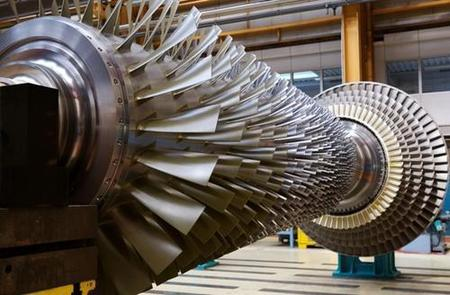
\includegraphics[width = 0.6\hsize]{./figures/bayesopt/Turbine-Blade}
\end{figure}

\end{frame}



\begin{frame}
\frametitle{Machine Learning Meta-Challenges}

\begin{itemize}
\item Machine learning models are getting more and more complicated
\\
\arrow Usually more parameters (e.g., deep neural networks)
\item Non-convex and stochastic optimization methods have
  meta-parameters that are difficult to tune (learning rates, momentum
  parameters, ...)
\end{itemize}
  \arrow Generally hard to apply modern techniques or reproduce
   results
\pause
\begin{myblock}{}
  Goal: Automate the selection of critical meta-parameters \\(see also:
  \cemph{Automated Machine Learning (AutoML)})
\end{myblock}
\end{frame}


%%%%%%%%%%%%%%%%%%%%%%%%%%%%%%%%%%%%%%%%%%%%%%%%%%%%%

\begin{frame}
\frametitle{Example: Deep Neural Networks}
\begin{figure}
\centering
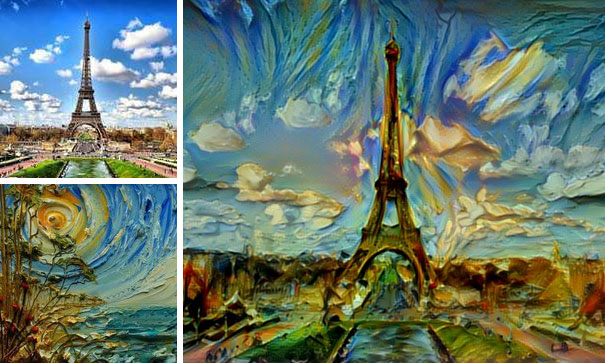
\includegraphics[width = 0.3\hsize]{./figures/bayesopt/nn_art}
\hfill
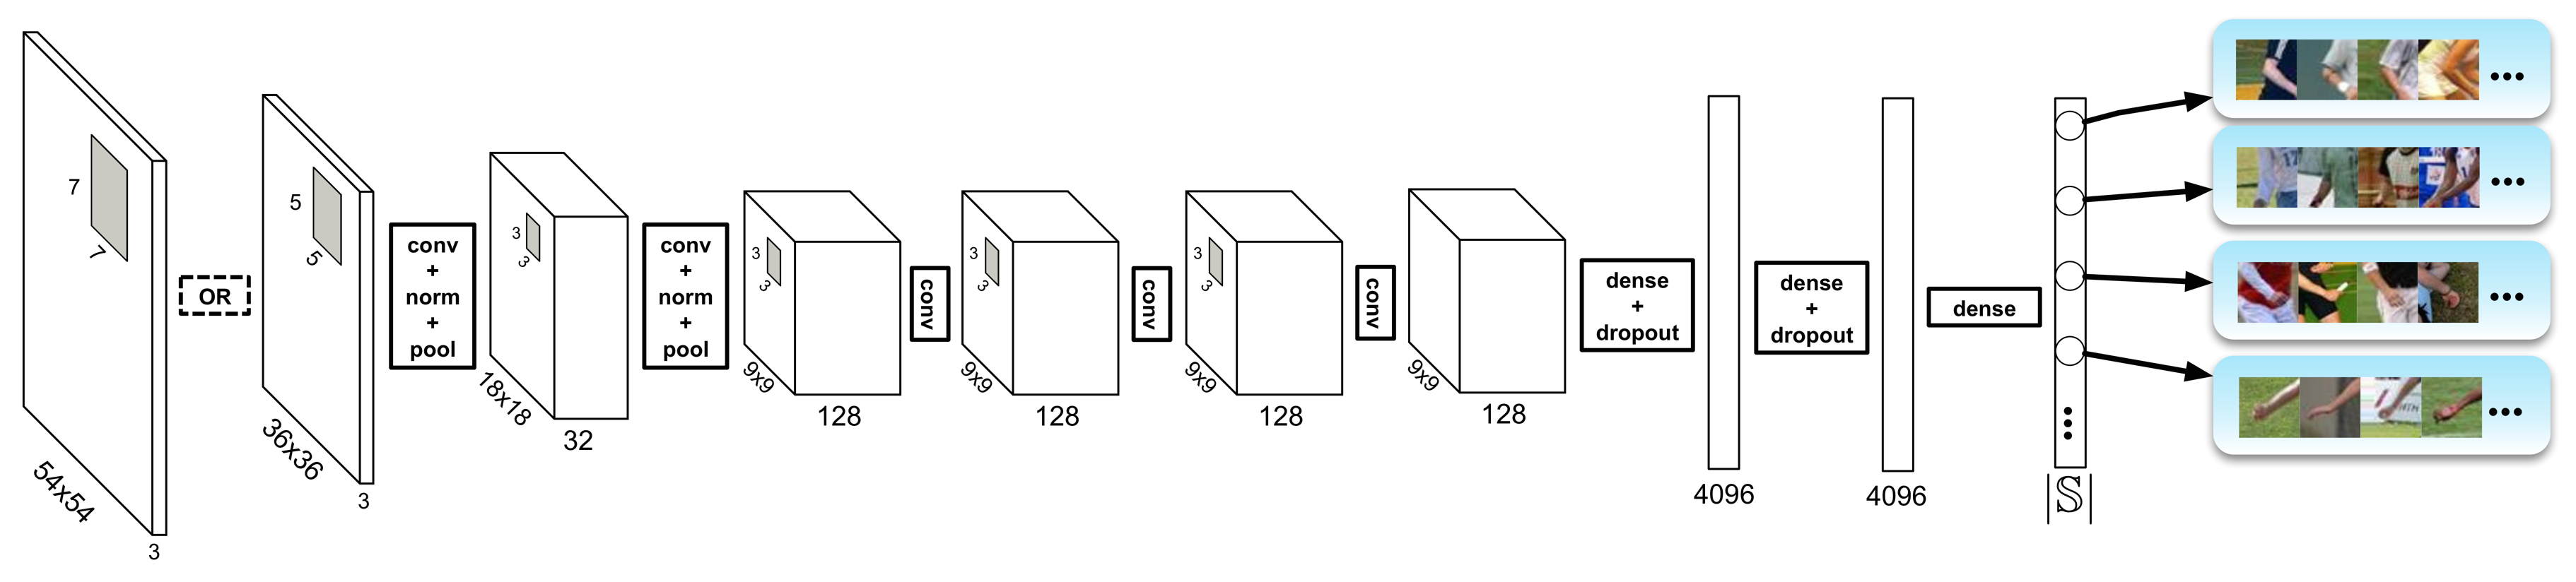
\includegraphics[width=0.65\hsize]{./figures/bayesopt/DCNN_model}
\end{figure}

Huge interest in large neural networks
\begin{itemize}
\item When well-tuned, very successful for visual object
identification, speech recognition, computational biology, ...
\item Huge investments by Google, Facebook, Microsoft, etc.
\item \calert{Many choices:} number of layers, weight regularization,
layer size, which nonlinearity, batch size, learning rate
schedule, stopping conditions
\end{itemize}
\end{frame}


\begin{frame}
\frametitle{Example: Online Latent Dirichlet Allocation}


\begin{figure}
\centering
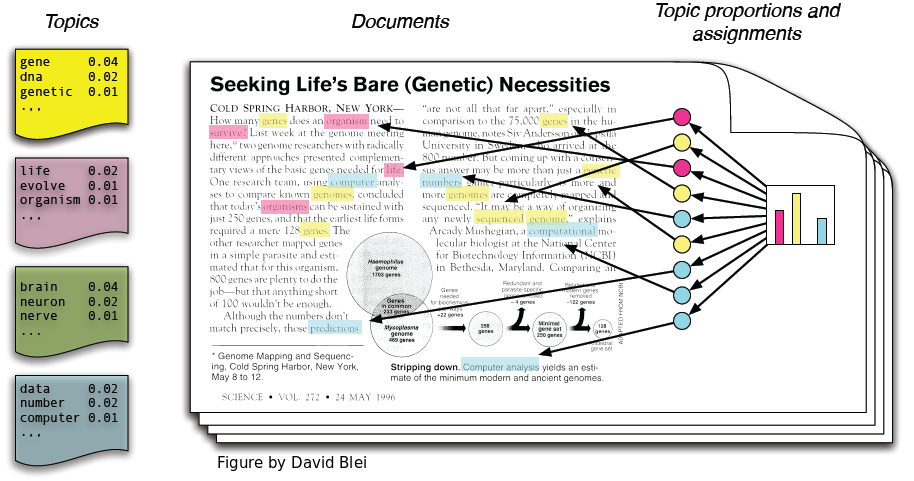
\includegraphics[height = 3cm]{./figures/bayesopt/lda}
\hfill
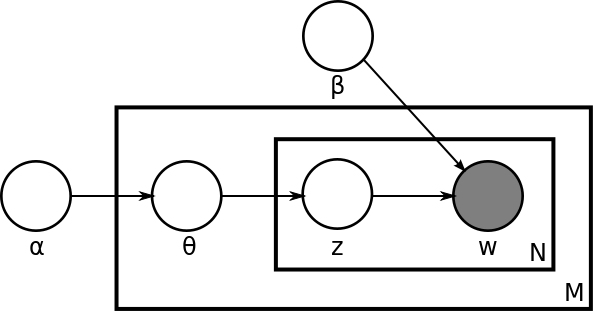
\includegraphics[height = 3cm]{./figures/bayesopt/gm_lda}
\end{figure}

\begin{itemize}
\item Hoffman et al. (2010): Approximate inference for \cemph{large-scale
  text analysis (topic modeling) with Latent Dirichlet Allocation}
\item Good empirical results when well tuned
\item \calert{Hyper-parameters} tricky to set: Dirichlet parameters, number of
  topics, learning rate schedule, batch size, vocabulary size, ...\nocite{Hoffman2010}
\end{itemize}
\end{frame}


\begin{frame}
\frametitle{Example: Classification of DNA Sequences}
\begin{figure}
\centering
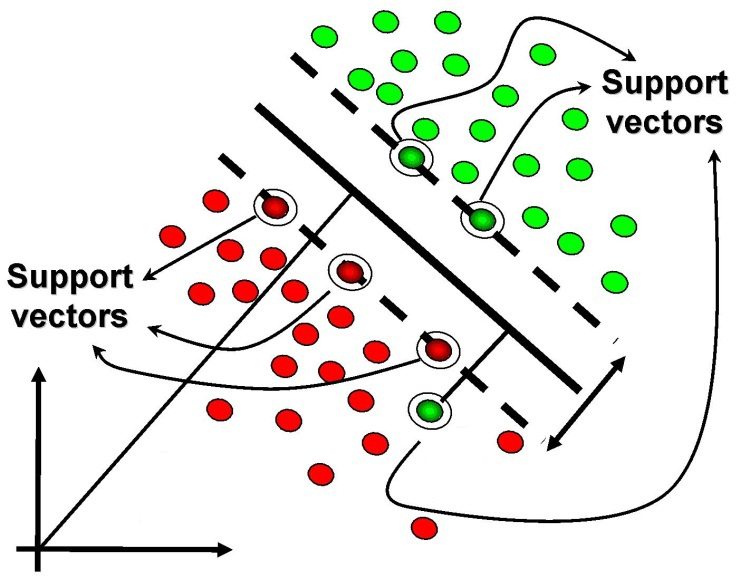
\includegraphics[height = 3cm]{./figures/bayesopt/SVM}
\hspace{5mm}
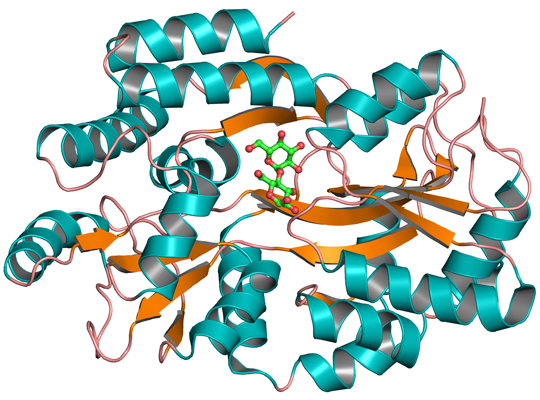
\includegraphics[height = 3cm]{./figures/bayesopt/protein}
\end{figure}

\begin{itemize}
\item Objective: Predict which DNA sequences will bind with which
  proteins
\item Miller et al. (2012):\nocite{Miller2012} \cemph{Latent Structural
  Support Vector Machine}
\item \calert{Hyper-parameters:} margin/slack parameter, entropy parameter,
  convergence criterion
\end{itemize}
\end{frame}




\begin{frame}
\frametitle{Search for Good Hyper-parameters}

\begin{itemize}
\item Define an objective function to evaluate the quality of the hyper-parameters
\begin{itemize}
\item Usually, we care about generalization performance
\item Cross validation to measure parameter quality
\end{itemize}
\pause
\item Standard search procedures:
\begin{itemize}
\item Manual tuning
\item Grid search
\item Random search (very simple, works surprisingly well)
\item Black magic
\end{itemize}
\pause
\item Painful:
\begin{itemize}
\item Evaluating the quality of the objective may be very expensive
  (e.g., time or money)\\
  \arrow Imagine we would need to run a GPU/TPU cluster for 2 weeks
\item Many training cycles
\item Possibly noisy
\end{itemize}
\end{itemize}
\end{frame}




\begin{frame}
\frametitle{Alternative Approach: Bayesian Optimization}
\begin{myblock}{Setting}
Globally optimize a black-box objective that is expensive to evaluate
(e.g., cross-validation error for a massive neural network)
\end{myblock}

We want to be smart about using the evaluations we have
\pause
\begin{itemize}[<+->]
\item Build a \cemph{probabilistic proxy model} for the objective using
  outcomes of past experiments as training data
\item We can predict the outcome of the next experiment using the proxy model, which is much \cemph{cheaper to evaluate}
%\item Use posterior predictive distribution of the probabilistic model
\item \cemph{Optimize cheap proxy} function to determine where to evaluate the true
  objective next
\item Standard proxy: \cemph{Gaussian process}
\end{itemize}
% \begin{myblock}{}
% The main insight:
% Make the proxy function exploit uncertainty to balance
% exploration against exploitation.

% \end{myblock}
\end{frame}

%%%%%%%%%%%%%%%%%%%%%%%%%%%%%%%%%%%%%%%%%%%%%%%%%%%%%

\begin{frame}
\frametitle{Setting (2)}
\begin{itemize}
\item Objective: Find global minimum of objective function $f$:
 $$\vec x_* = \arg\min_{\vec x} f(\vec x)$$
\item We can evaluate the objective $g$ pointwise, but do not have an easy
  functional form or gradients; observations may be noisy
\item \calert{Evaluating $f$ is costly} (e.g., train a massive deep network)
\end{itemize}

\begin{figure}
\centering
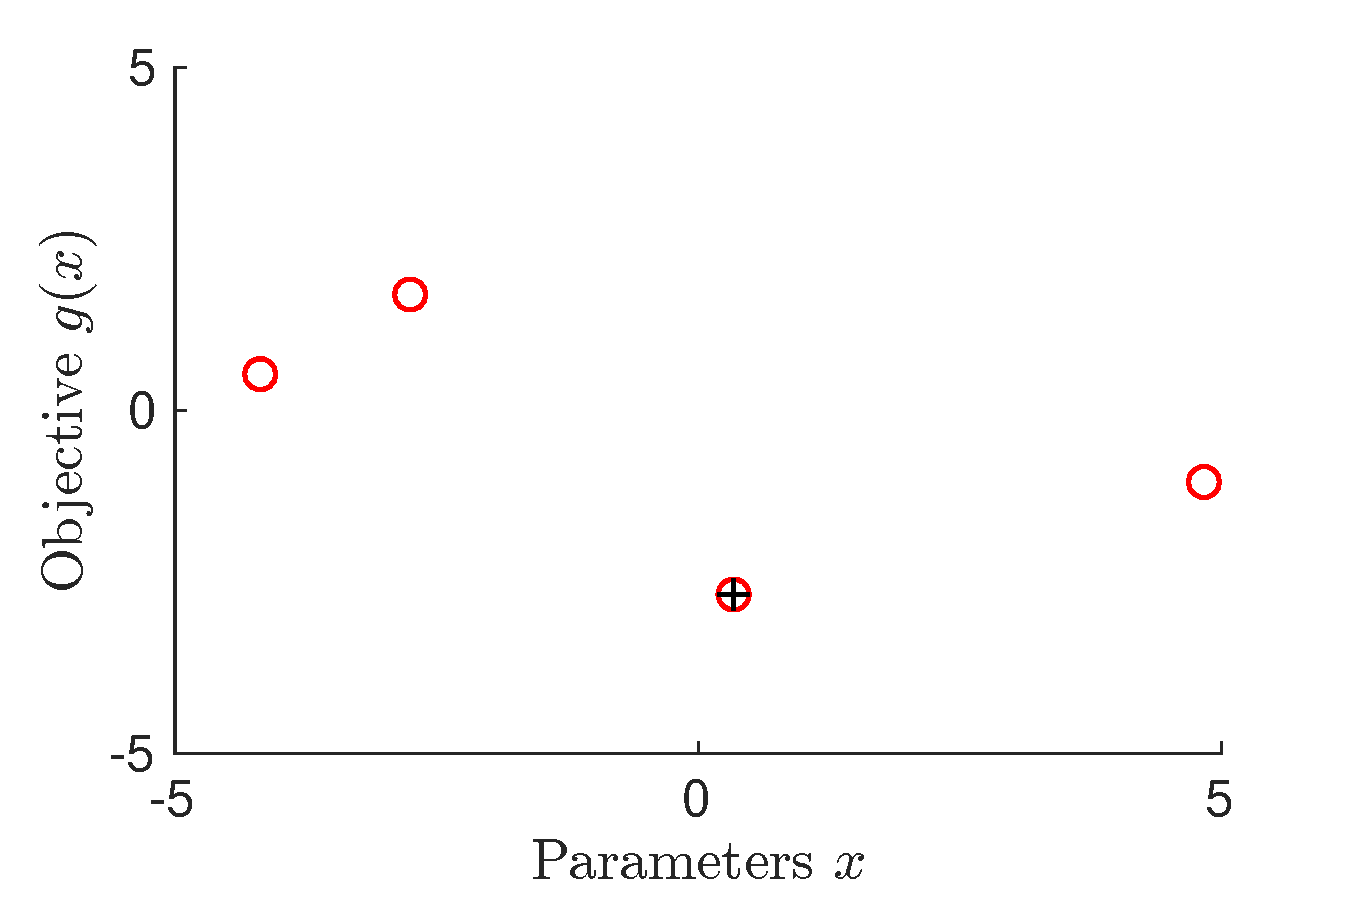
\includegraphics[height = 4cm]{./figures/bayesopt/bo_init}
\end{figure}
\end{frame}






% \begin{frame}{Recap: Prospecting for gold}
% First choose location to prospect at $p$,
% then choose location to mine $m$. \pause
% \begin{enumerate}[{\hspace{0.3cm}Step} 1:]
% \item $U(\vx, d_p, m, p) = -c_p + x_m$ \pause
% \item $\Exp{p(\vx, d_p)}{U(\vx, d_p, m, p)} = \Exp{p(\vx, d_p)}{-c_p + x_m}$ \pause
% \item $\text{action} = \argmax_{\text{actions}} \Exp{p(\vx, d_p)}{U(\vx, d_p, m, p)}$ \end{enumerate}

% % \begin{align}
% % U(\vx, d_p, m, p) &= -c_p + x_m \\
% % \Exp{p(\vx, d_p)}{U(\vx, d_p, m, p)} &= \Exp{p(\vx, d_p)}{-c_p + x_m} \\
% % \end{align}
% \pause
% \vspace{0.4cm}
% Trick is to realise that
% \begin{align}
% m(d_p) = \argmax_n \Exp{p(\vx\given d_p)}{x_n} = \argmax_n \mu_n'(d_p)
% \end{align}
% \pause
% so...
% \begin{align}
% U(\vx, d_p, p) &= -c_p + x_{m(d_p)} \\
% \Exp{p(\vx, d_p)}{U(\vx, d_p, p)} &= -c_p + \Exp{p(d_p)}{\Exp{p(\vx\given d_p)}{x_{m(d_p)}}} \\
% &= -c_p + \Exp{p(d_p)}{\max_{n}\mu_n'}
% \end{align}
% \end{frame}


\begin{frame}{Bayesian optimisation}
Let's phrase BayesOpt using decision theory:
\begin{align}
L(f, \{\vx_n\}_{n=1}^N) = Nc + \min_{1 \leq n \leq N} f(\vx_n)
\end{align}
(Optimisers are pessimists, they talk about loss instead of utility)
\pause
\begin{itemize}
\item We decide how many evaluations we want to do $N$
\item We decide where to evaluate $f(\cdot)$
\item We incur a cost $c$ for each evaluation
\item We reduce loss by finding a lower $f(\vx)$
\end{itemize}
\end{frame}


\begin{frame}{Bayesian optimisation -- decision theory}
For 3 observations:
\begin{align}
\{\vx_1^*, \vx_2^*(\data_1), \vx_3^*(\data_2)\} = \argmin_{\{\vx_n\}_{n=1}^3} \Exp{p(f)}{Nc + \min_{1\leq n\leq N} f(\vx_n)}
\end{align}
\pause
Remember: actions $\vx_2$ and $\vx_3$ can depend on the data we observe. The data are observations of the GP $\data = \{\vx_n, f(\vx_n)\}_{n=1}^N$.
\pause
\begin{align}
\vx_1^* = -Nc + \argmin_{\vx_1} \Exp{f}{\min_{\vx_2} \Exp{f\given \data_1}{\min_{\vx_3} \Exp{f\given \data_2}{\min_{1 \leq n \leq 3} \{f(\vx_n)\}}}}
\end{align}
\end{frame}


\begin{frame}{Computational difficulties}
\begin{align*}
\vx_1^* = -Nc + \argmin_{\vx_1} \Exp{f}{\min_{\vx_2} \Exp{f\given \data_1}{\min_{\vx_3} \Exp{f\given \data_2}{\min_{1 \leq n \leq 3} \{f(\vx_n)\}}}}
\end{align*}

\vspace{0.3cm}

\pause

This is \emph{very} difficult to evaluate.
\begin{itemize}
\item Difficult optimisations: closed-form optimum cannot be found
\item Expectations of non-closed-form expressions
\item Optimisations of expectations of non-closed-form expressions
\end{itemize}

\vspace{0.4cm} \pause

Alternative approaches:
\begin{itemize}
\item Can try to approximate these quantities (fun to try for small-scale examples)
\item Heuristic approaches
\end{itemize}
\end{frame}



\begin{frame}{How to design a heuristic}
In BayesOpt, heuristic is called the \emph{acquisition function}. Instead of maximising the utility (or minimising loss), we maximise the acquisition function.
\pause
\begin{itemize}
\item Computational constraint: Only use posterior of GP given \emph{current} observations to choose current action \pause
\item Desired behaviour: Some sort of a trade-off between \emph{exploration} and \emph{exploitation}. \pause
\begin{itemize}
\item Want to try inputs that are different (exploration)
\item Want to focus on areas that are likely to have high values (exploitation)
\end{itemize}
\end{itemize}
\end{frame}

% \begin{itemize}
% \item Computational constraint: Only use posterior of GP given \emph{current} observations
% \item Desired behaviour: Some sort of a trade-off between \emph{exploration} and \emph{exploitation}.
% \end{itemize}
% posteiror of


\begin{frame}{Inadequate acquisition functions}
Two inadequate acquisition functions:
\begin{itemize}
  \item Minimise posterior mean (pure exploitation)
  \item Maximise posterior variance (pure exploration)
\end{itemize}
\begin{figure}
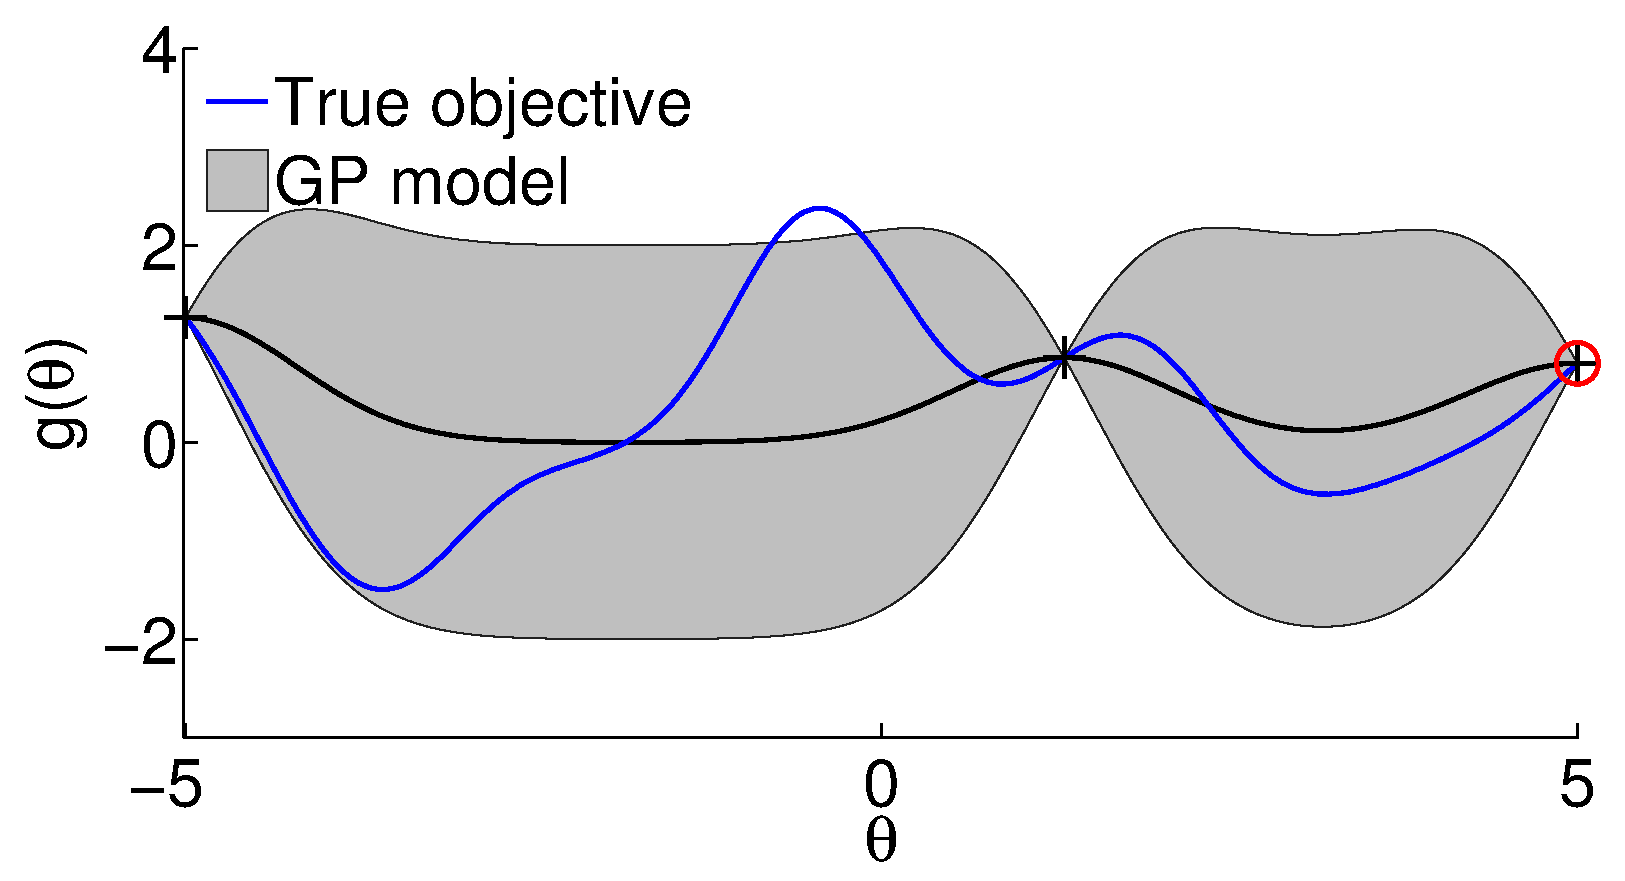
\includegraphics[height = 5cm]{./figures/bayesopt/BOa3}
\end{figure}
\end{frame}



\begin{frame}
  \frametitle{Common acquisition functions}

\begin{itemize}
\item For all $\vec x\in\R^D$ the GP posterior gives a predictive mean
  $\mu(\vec x)$ variance $\sigma^2(\vec x)$ of $g(\vec x)$
\item Define
$$
\green{\gamma(\vec x) = \frac{f(\vec x_{\text{best}}) - \mu(\vec
  x)}{\sigma(\vec x)}}
$$
\pause
\item  \emph{Probability of Improvement (Kushner 1964)\nocite{Kushner1964}:}
$$
\alpha_{\text{PI}}(\vec x) = \Phi(\green{\gamma(\vec x)})
$$
\item \emph{Expected Improvement (Mockus 1978)\nocite{Mockus1978}:}
$$
\alpha_{\text{EI}}(\vec x) = \sigma(\vec x)\big(\green{\gamma (\vec x)}\Phi(\green{\gamma(\vec
x)}) + \gaussx{\green{\gamma(\vec x)}}{0}{1}\big)
$$
\item \emph{GP Lower Confidence Bound (Srinivas et al., 2010):\nocite{Srinivas2010}}
$$
\alpha_{\text{LCB}}(\vec x) = - (\mu(\vec x) - \kappa\sigma(\vec
x))\,,\quad\kappa > 0
$$
\end{itemize}
\end{frame}






\begin{frame}
\frametitle{Probability of Improvement (1)}
\begin{columns}
\column{0.5\hsize}
\begin{figure}
\centering
\includegraphics[width = \hsize]{./figures/bayesopt/bo_PI_samples_no_slack}
\end{figure}
\column{0.5\hsize}
\begin{itemize}
\item \cemph{Idea:} Determine the probability that $\vec x_*$ leads to a better
  function value than the currently best one $f(\vec x_{\text{best}})$
\item Sampling-based setting: Sample $N$ functions $f_i$; at every
  input $\vec x$ compute a Monte-Carlo estimate
\end{itemize}
\end{columns}

\begin{align*}\alpha_{\text{PI}}(\vec x) &= p(f(\vec x) < f(\vec
 x_{\text{best}}))\approx \frac{1}{N}\sum\nolimits_{i=1}^N \delta\big(f_i(\vec x) <
  f(\vec x_{\text{best}})\big)
 \end{align*}
\pause
\arrow Can lead to continued exploitation in an $\epsilon$-region around $\vec
x_{\text{best}}$.\\
\pause
\arrow Introduce a ``slack variable'' $\xi$ for more aggressive exploration
\end{frame}

%%%%%%%%%%%%%%%%%%%%%%%%%%%%%%%%%%%%%%%%%%%%%%%%%%%%%
\begin{frame}
\frametitle{Probability of Improvement (2)}
\begin{figure}
\centering
\includegraphics[width = 0.48\hsize]{./figures/bayesopt/bo_PI_samples_no_slack}
\hfill
\includegraphics[width = 0.48\hsize]{./figures/bayesopt/bo_PI_samples_with_slack}
\end{figure}
\vspace{-5mm}
\begin{itemize}
\item Look at a minimum improvement of $\colchar{$\xi$}{blue}>0$:
 $$\alpha_{\text{PI}}(\vec x) = p(f(\vec x) < f(\vec x_{\text{best}})\colchar{$-\xi$}{blue}) \approx \frac{1}{N}\sum\nolimits_{i=1}^N \delta\big(f_i(\vec x) < f(\vec x_{\text{best}})\colchar{$-\xi$}{blue}\big)$$
\item If $f\sim GP$ and $p(f(\vec x)) = \gauss{\mu(\vec
    x)}{\sigma(\vec x)}$:
\begin{align*}
\alpha_{\text{PI}}(\vec x) =  \Phi(\gamma(\vec x, \xi))\,,\qquad
\gamma(\vec x, \xi) = \frac{f(\vec x_{\text{best}}) \colchar{$- \xi$}{blue} - \mu(\vec
  x)}{\sigma(\vec x)}
\end{align*}
\end{itemize}


\end{frame}
%%%%%%%%%%%%%%%%%%%%%%%%%%%%%%%%%%%%%%%%%%%%%%%%%%%%%
%\input{pi_example}
%%%%%%%%%%%%%%%%%%%%%%%%%%%%%%%%%%%%%%%%%%%%%%%%%%%%%

\begin{frame}
\frametitle{Expected Improvement}
\begin{columns}

\column{0.5\hsize}
\begin{itemize}
\item \cemph{Idea:} Quantify the \cemph{amount of improvement}
\item Sampling-based scenario, where $f_i\sim p(f)$:
\begin{align*}
\alpha_{\text{EI}}(\vec x) = \E[ \max\{0, f(\vec x_{\text{best}}) - f(\vec
x)\}] \\
\approx \frac{1}{N} \sum_{i=1}^N \max \{0, f(\vec x_{\text{best}}) -  f_i(\vec x) \}
\end{align*}
\end{itemize}
\column{0.45\hsize}
\begin{figure}
\centering
\includegraphics[width = \hsize]{./figures/bayesopt/bo_EI_samples}
\end{figure}
\end{columns}

\begin{itemize}
\item If $f\sim GP$, we have a closed-form expression:
\begin{align*}
\alpha_{\text{EI}}(\vec x) = \sigma(\vec x)\big(\gamma (\vec x)\Phi(\gamma(\vec
x)) + \gaussx{\gamma(\vec x)}{0}{1}\big)
\end{align*}
\item Slack-variable approach also possible (similar to PI)~\nocite{Lizotte2008,Brochu2009}
\end{itemize}
\end{frame}

%%%%%%%%%%%%%%%%%%%%%%%%%%%%%%%%%%%%%%%%%%%%%%%%%%%%%

\begin{frame}
\frametitle{GP-Lower Confidence Bound (1)}
\begin{figure}
\centering
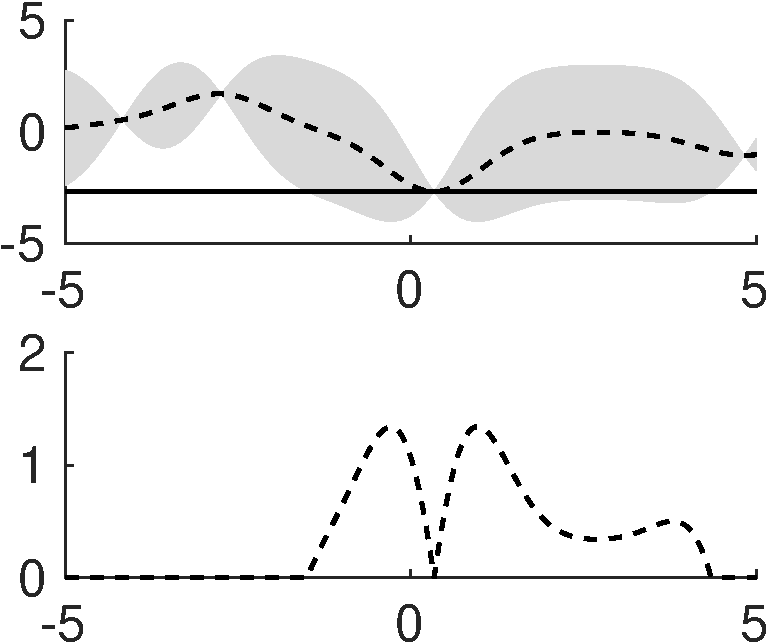
\includegraphics[height = 4cm]{./figures/bayesopt/bo_example_ucb}
\end{figure}
\begin{itemize}
\item Use the predictive mean $\mu(\vec x) $ and variance
  $\sigma^2(\vec x)$ of the GP prediction directly for
  targeted exploration by means of the acquisition function
\begin{align*}
\alpha_{\text{LCB}}(\vec x_t) = -\big( \mu(\vec x_t) - \sqrt{\kappa}\sigma(\vec x_t)\big)
\end{align*}
% In practice: Use
% $\max \{0, g(\vec x_{\text{best}}) - \alpha_{\text{LCB}}(\vec x_t) \}$
%max(fbest_LCB - UCB(-kappa, post_mean_LCB, sqrt(post_var_LCB)),0);

\end{itemize}
\end{frame}

%%%%%%%%%%%%%%%%%%%%%%%%%%%%%%%%%%%%%%%%%%%%%%%%%%%%%

\begin{frame}
\frametitle{GP-Lower Confidence Bound (2)}
\begin{figure}
\centering
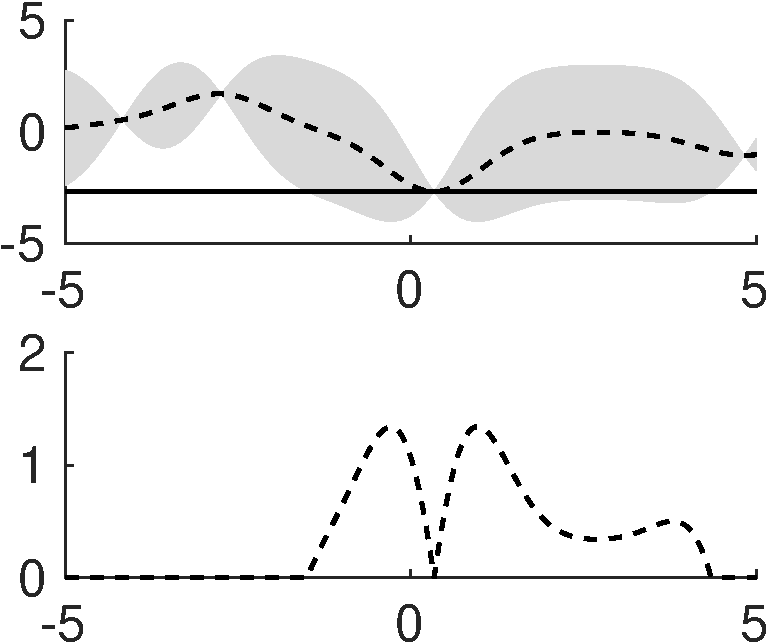
\includegraphics[height = 4cm]{./figures/bayesopt/bo_example_ucb}
\end{figure}
\begin{itemize}
\item More generally, we can get regret bounds for iteration-dependent
  $\kappa$ (Srinivas et al., 2010)\nocite{Srinivas2010}
\begin{align*}
  \alpha_{\text{LCB}}(\vec x_t) = -\big(\mu(\vec x_{t}) - \sqrt{\kappa_t}\sigma(\vec x_{t})\big)
\end{align*}
where $\kappa_t\in\mathcal O(\log t)$ grows with the iteration $t$
\\
\arrow Continue exploration
\end{itemize}
\end{frame}





\begin{frame}
\frametitle{Bayesian Optimization: Illustration}


\onslide*<1>{
\begin{figure}
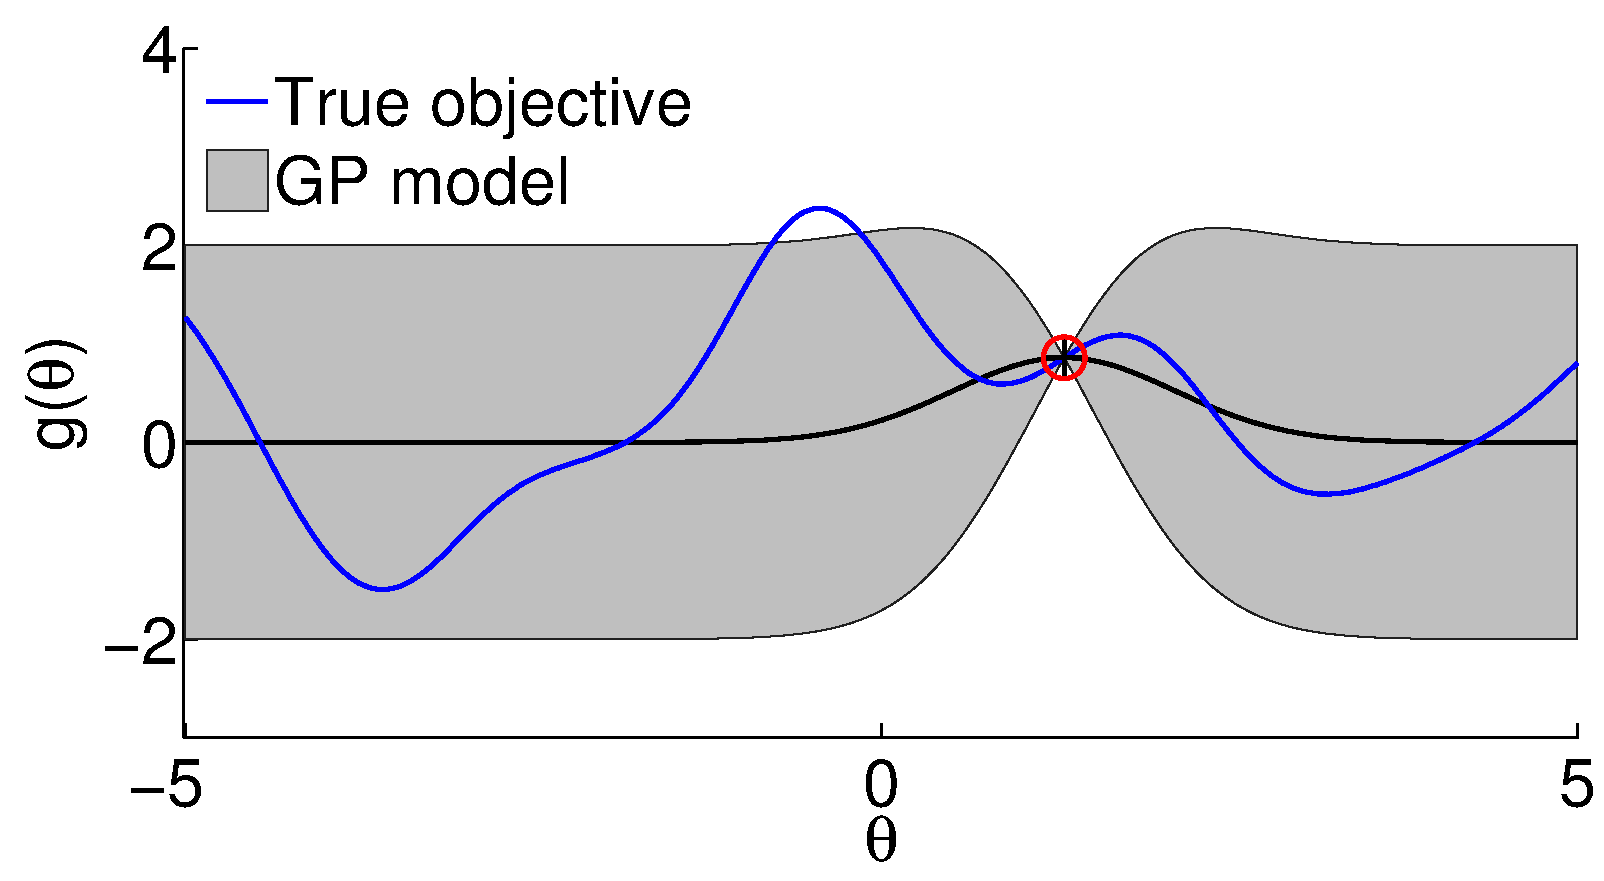
\includegraphics[height = 5cm]{./figures/bayesopt/BOa1}\hspace{1.2mm}
\end{figure}
}
\onslide*<2>{
\begin{figure}
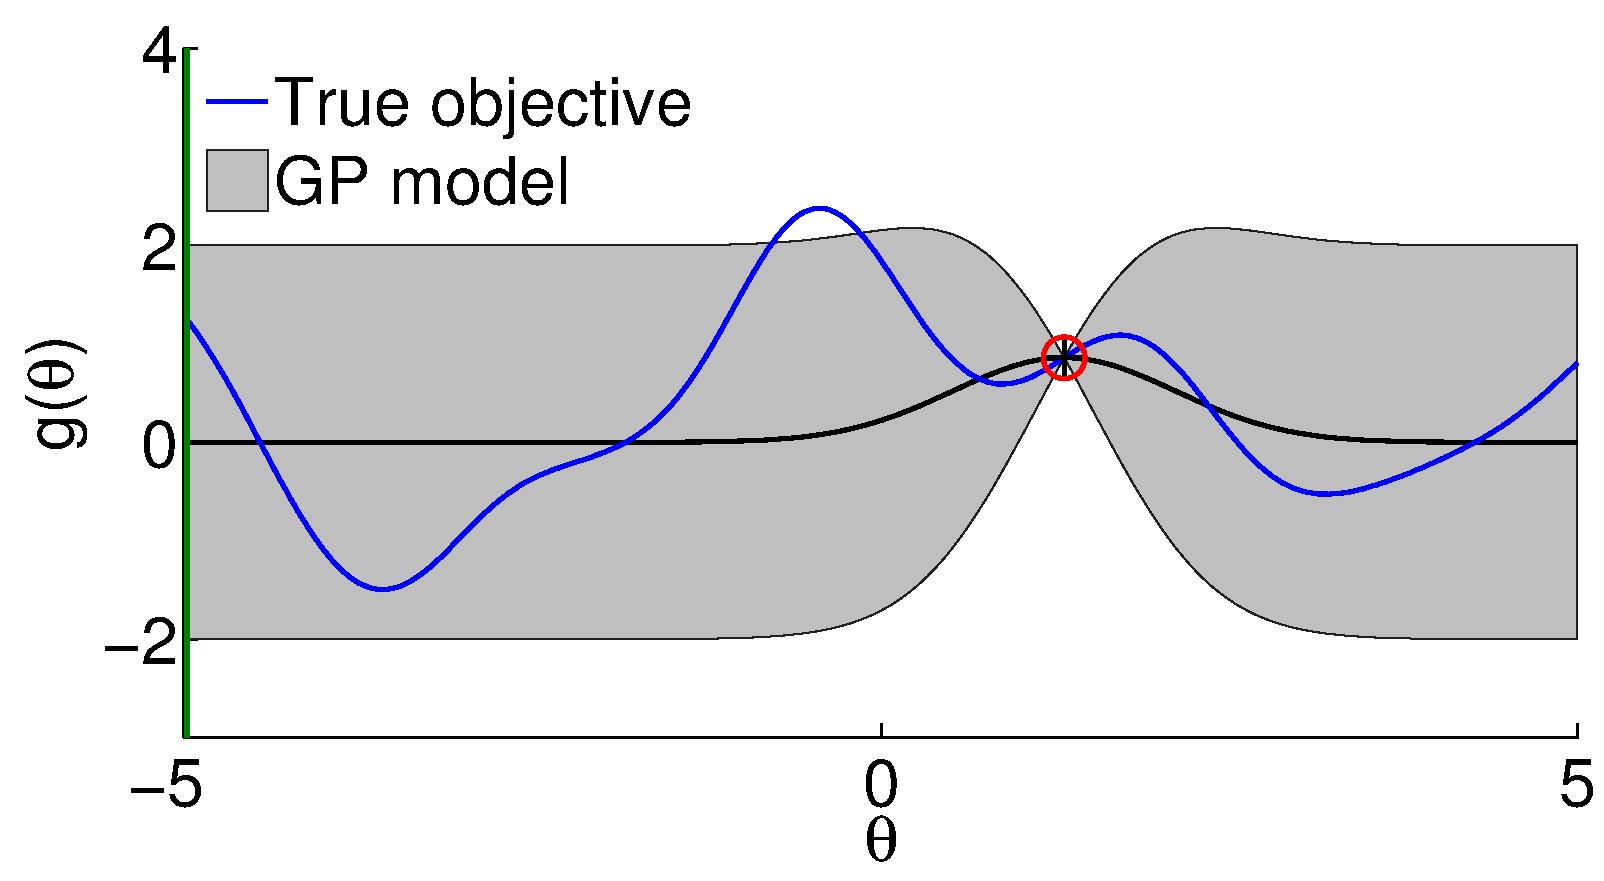
\includegraphics[height = 5cm]{./figures/bayesopt/BOb1}\hspace{1.2mm}
\end{figure}
}
\onslide*<3>{
\begin{figure}
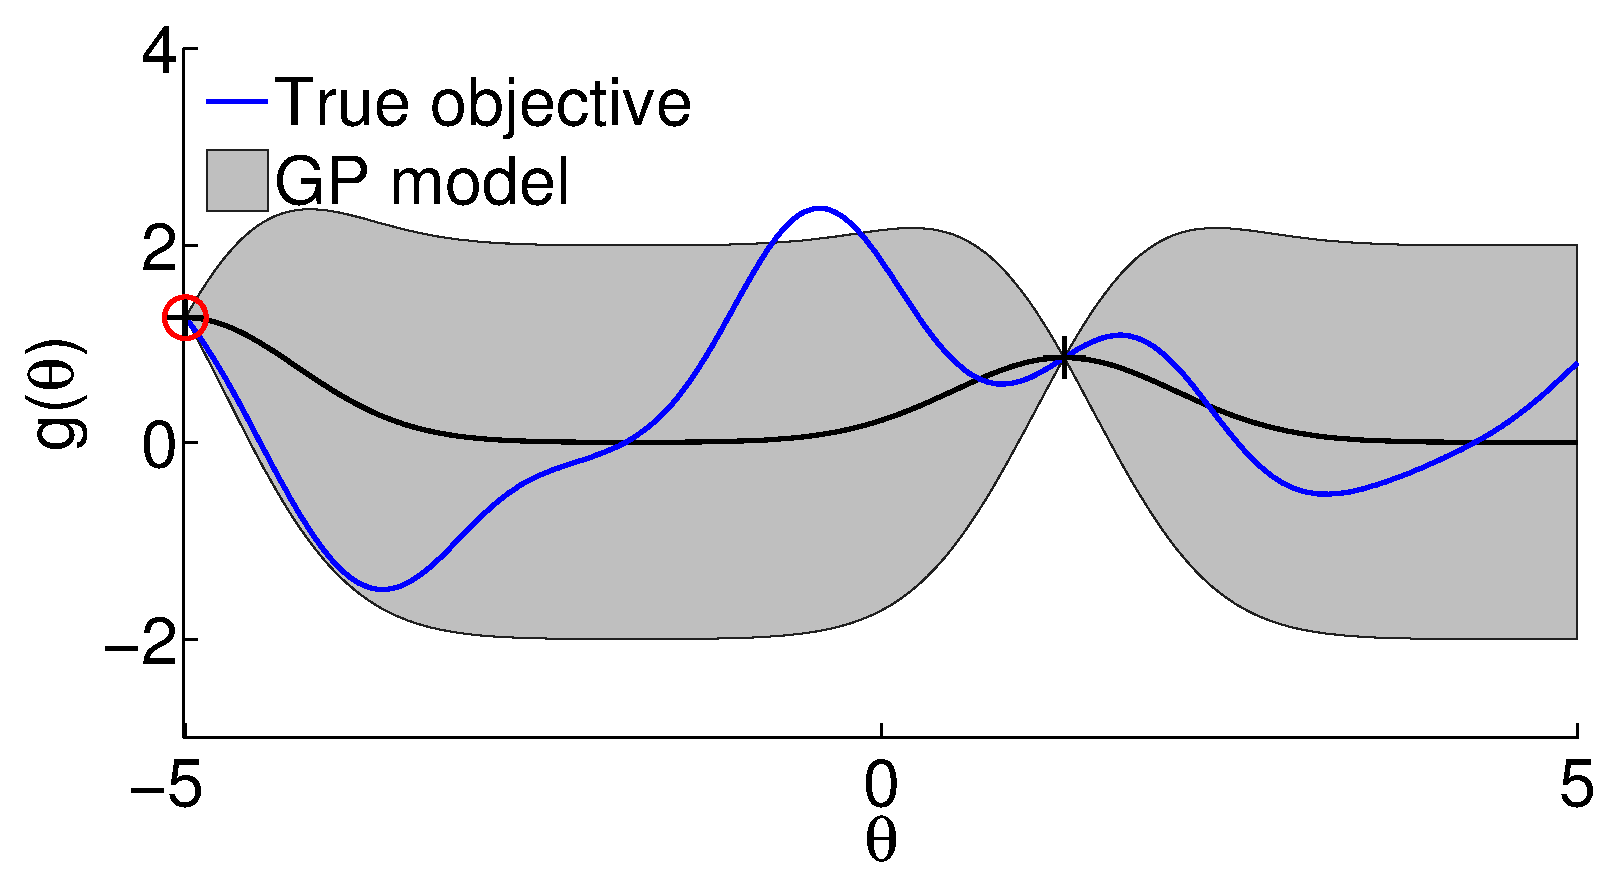
\includegraphics[height = 5cm]{./figures/bayesopt/BOa2}\hspace{1.2mm}
\end{figure}
}
\onslide*<4>{
\begin{figure}
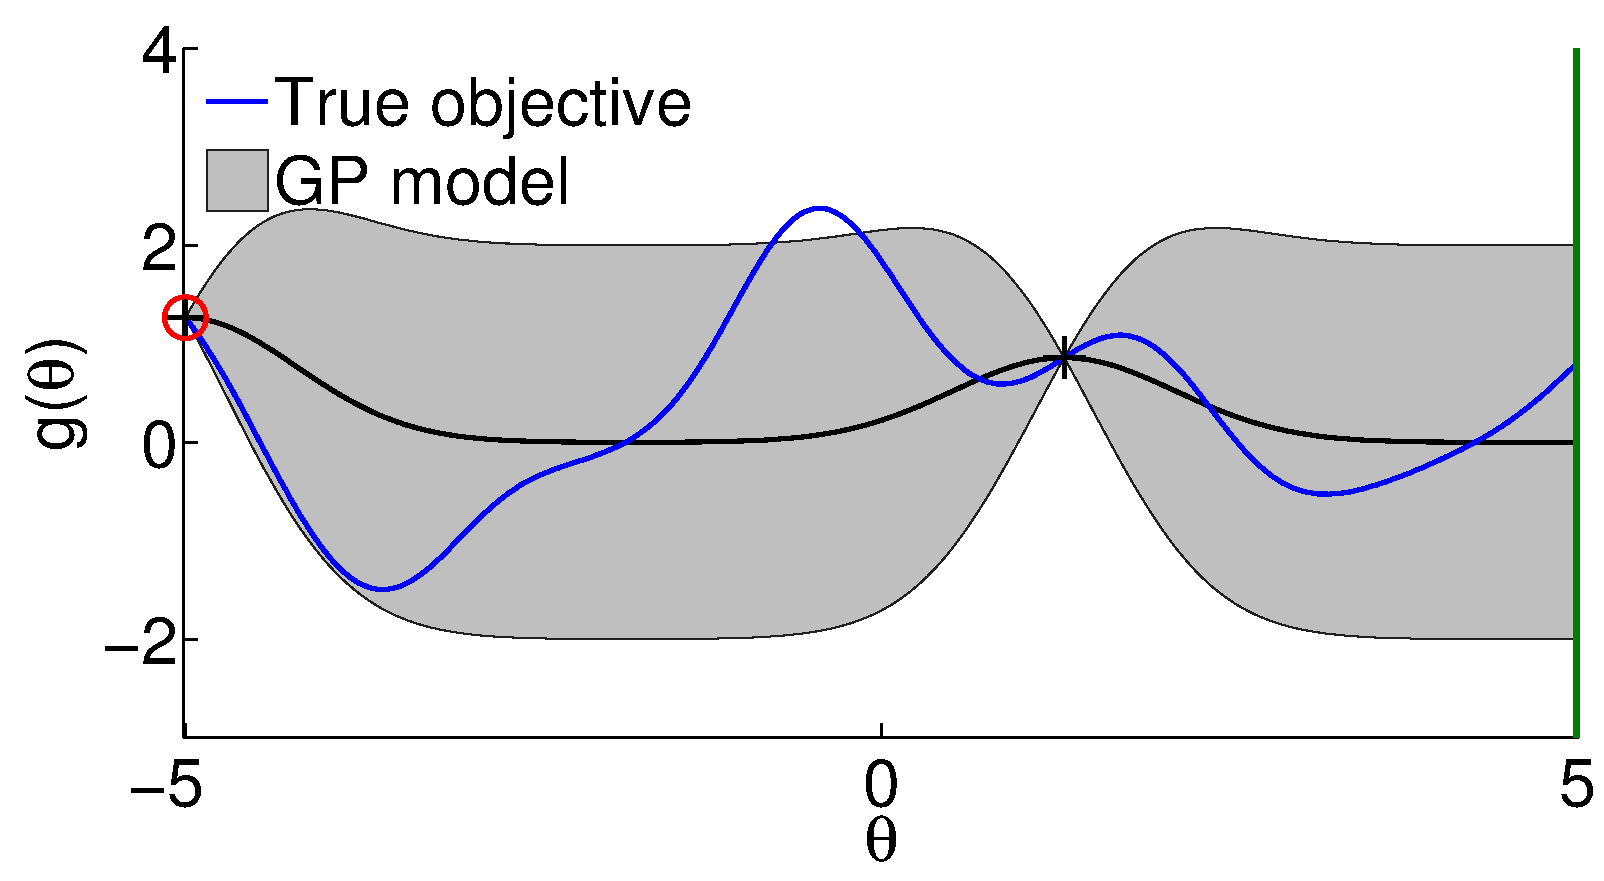
\includegraphics[height = 5cm]{./figures/bayesopt/BOb2}\hspace{1.2mm}
\end{figure}
}
\onslide*<5>{
\begin{figure}
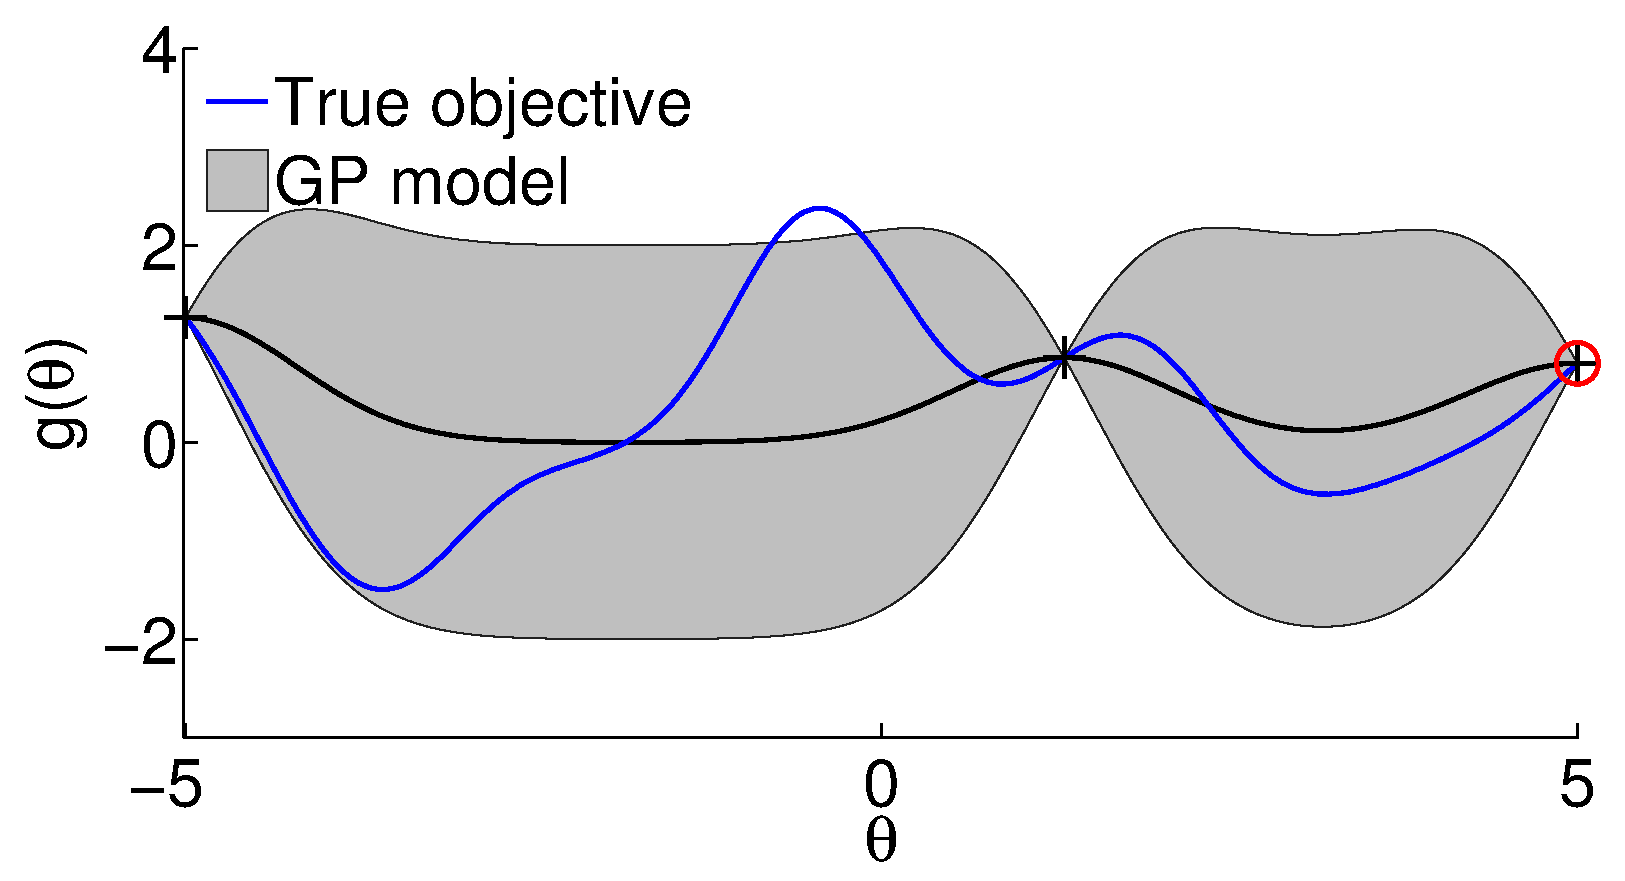
\includegraphics[height = 5cm]{./figures/bayesopt/BOa3}
\end{figure}
}
\onslide*<6>{
\begin{figure}
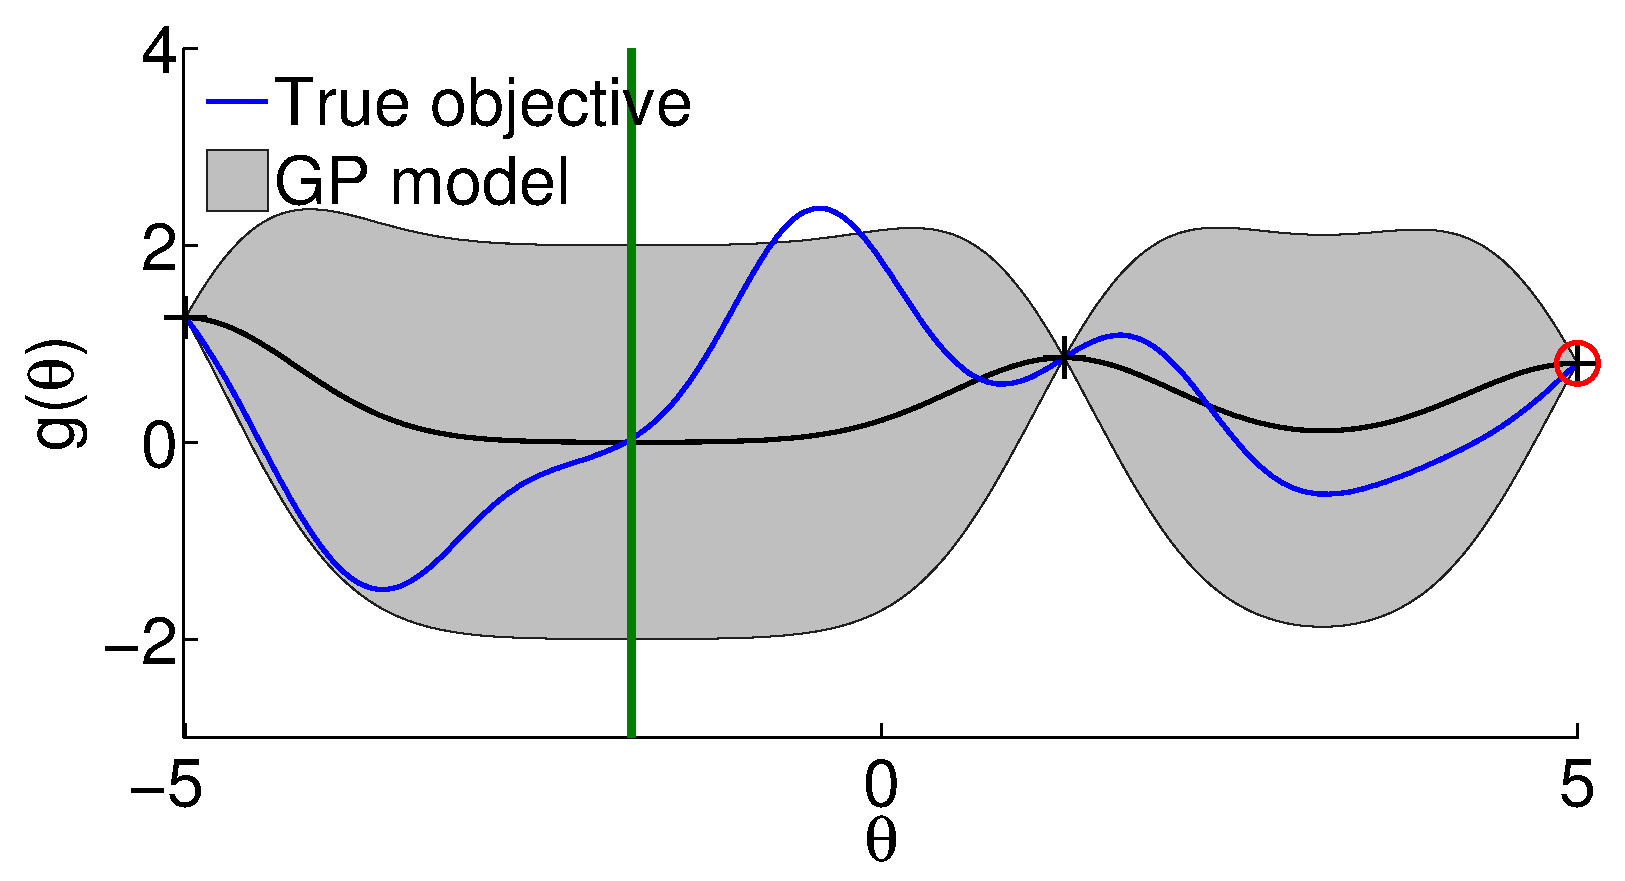
\includegraphics[height = 5cm]{./figures/bayesopt/BOb3}
\end{figure}
}
\onslide*<7>{
\begin{figure}
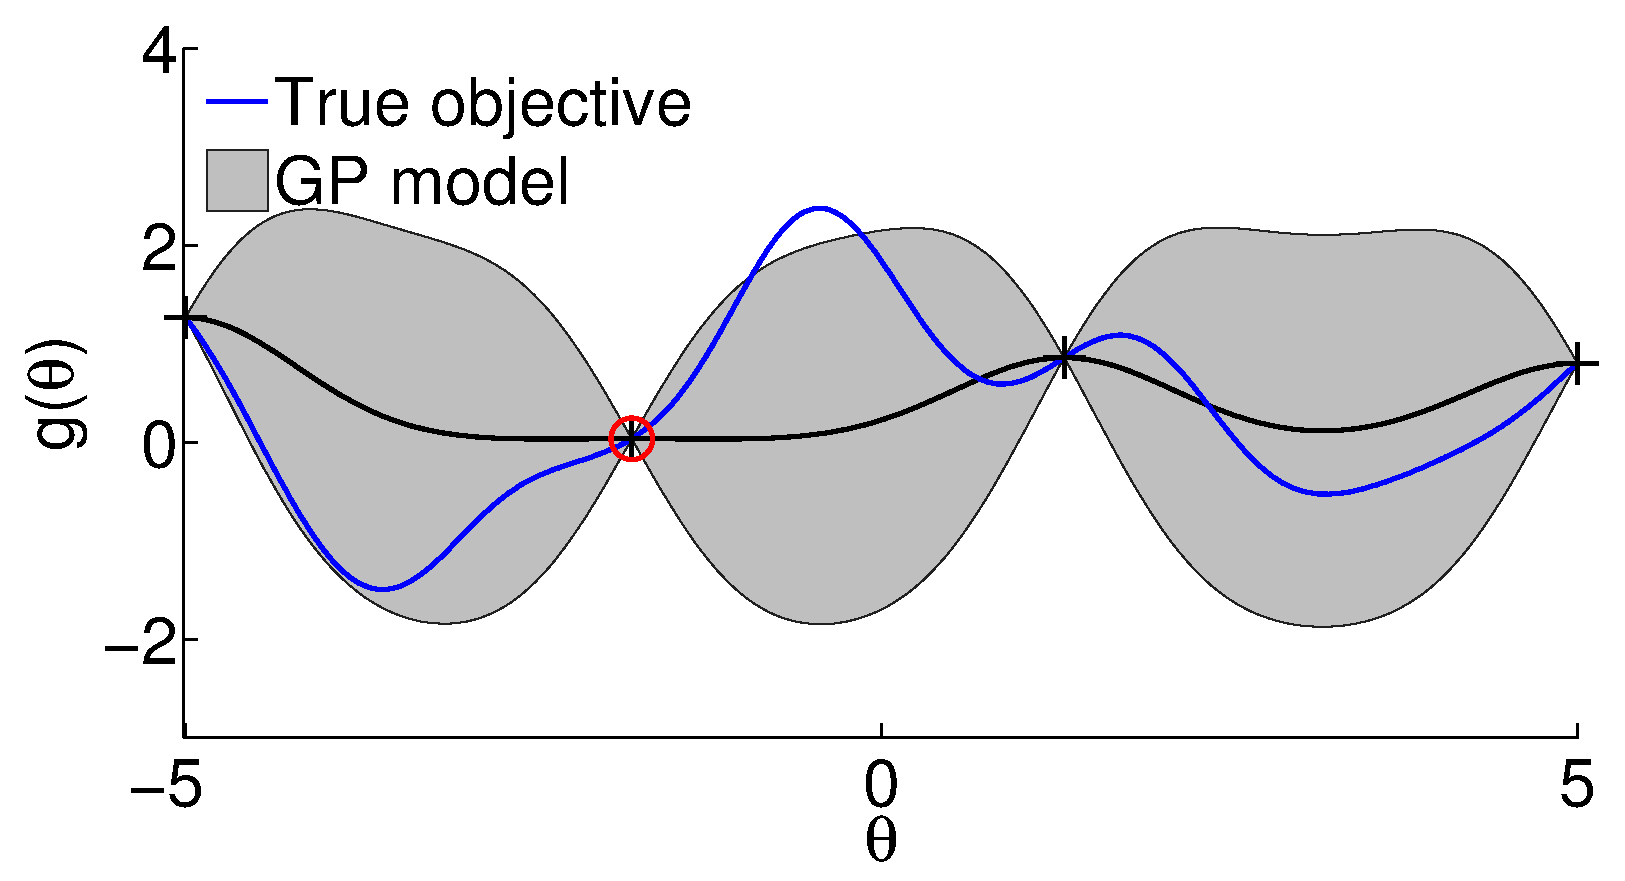
\includegraphics[height = 5cm]{./figures/bayesopt/BOa4}
\end{figure}
}
\onslide*<8>{
\begin{figure}
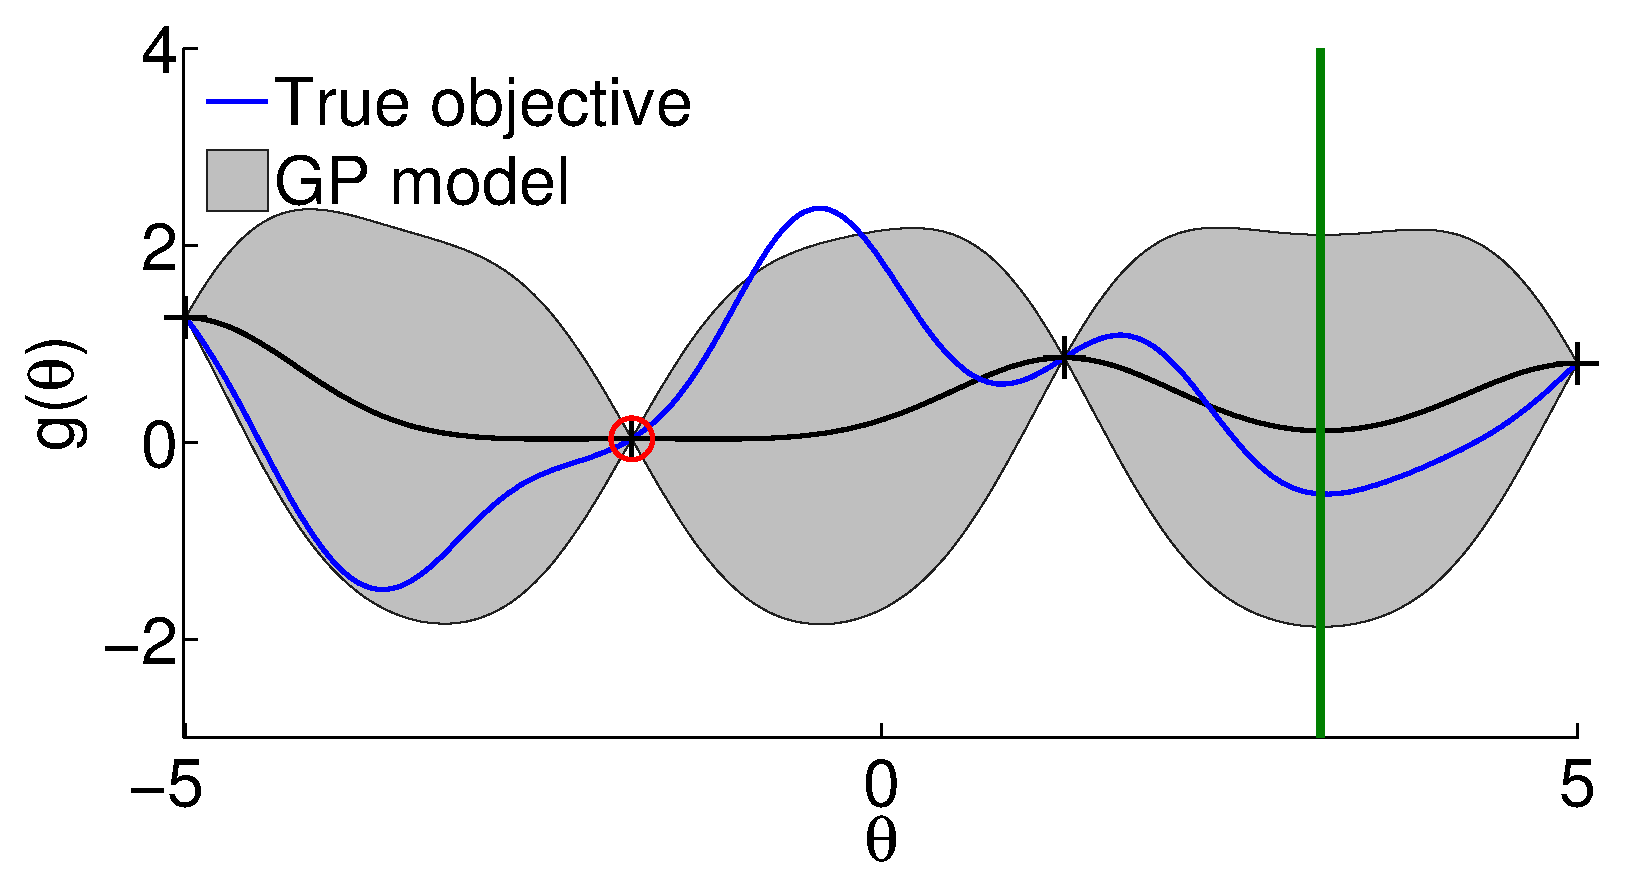
\includegraphics[height = 5cm]{./figures/bayesopt/BOb4}
\end{figure}
}
\onslide*<9>{
\begin{figure}
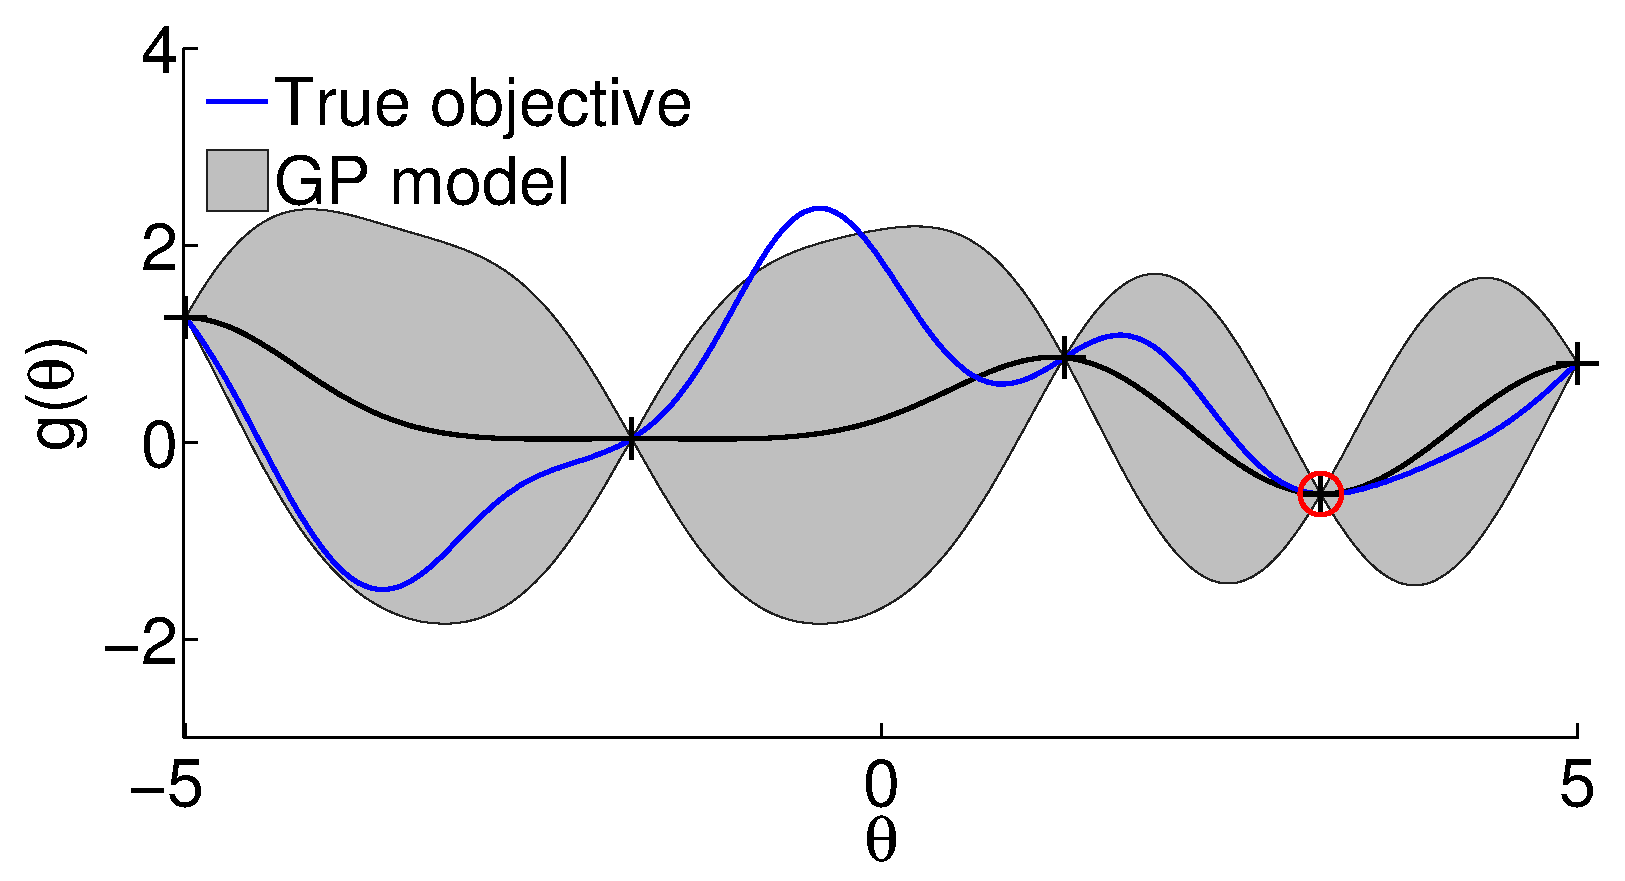
\includegraphics[height = 5cm]{./figures/bayesopt/BOa5}
\end{figure}
}
\onslide*<10>{
\begin{figure}
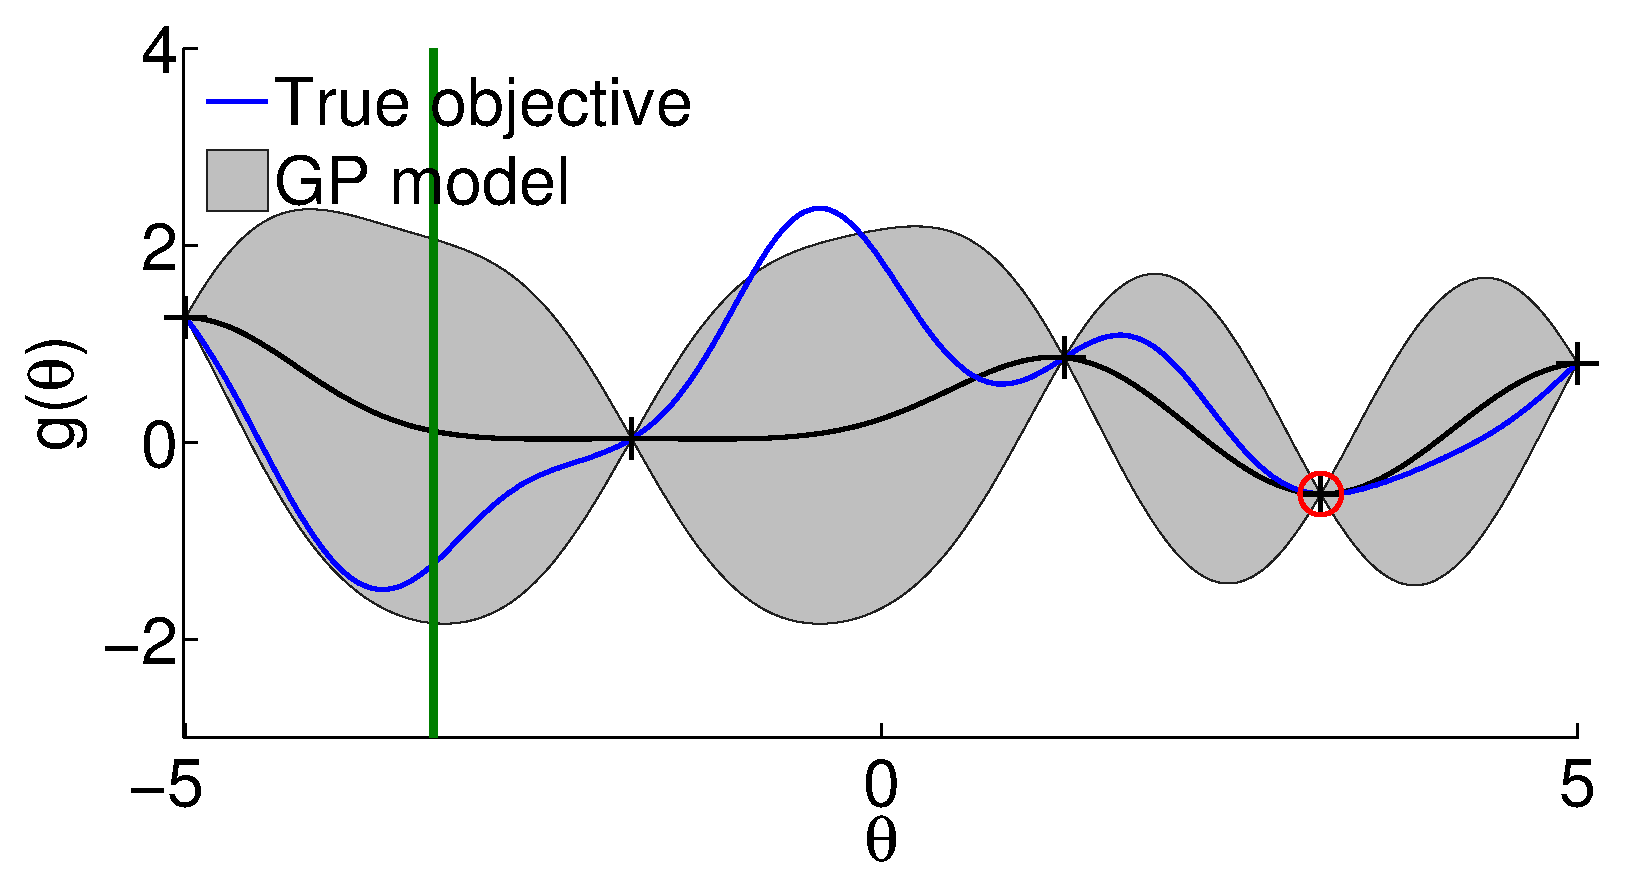
\includegraphics[height = 5cm]{./figures/bayesopt/BOb5}
\end{figure}
}
\onslide*<11>{
\begin{figure}
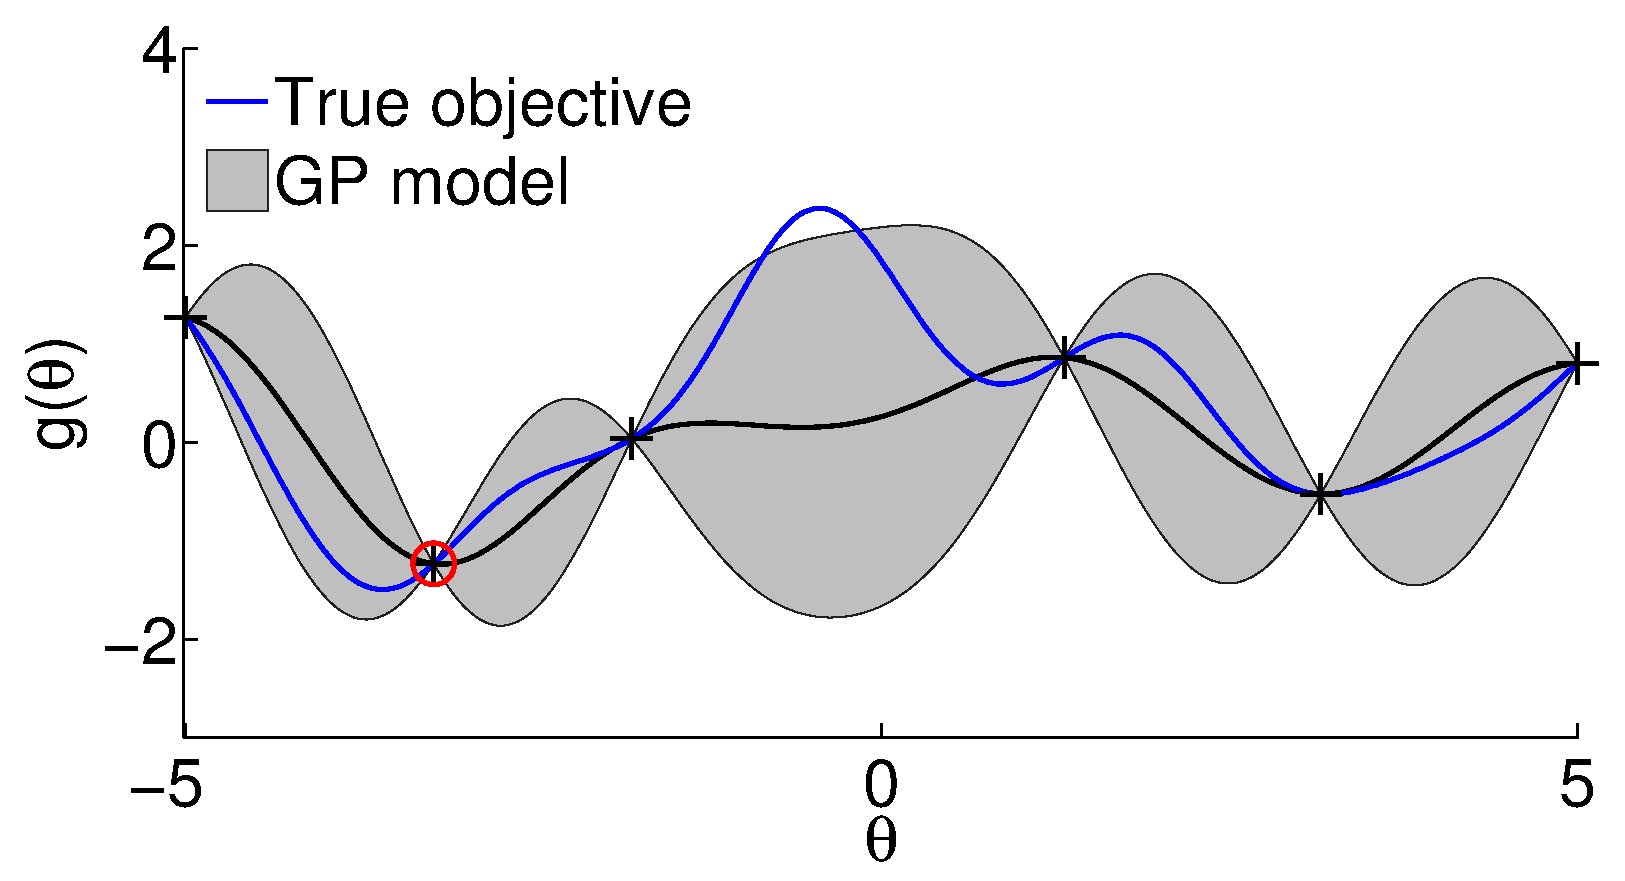
\includegraphics[height = 5cm]{./figures/bayesopt/BOa6}
\end{figure}
}
\onslide*<12>{
\begin{figure}
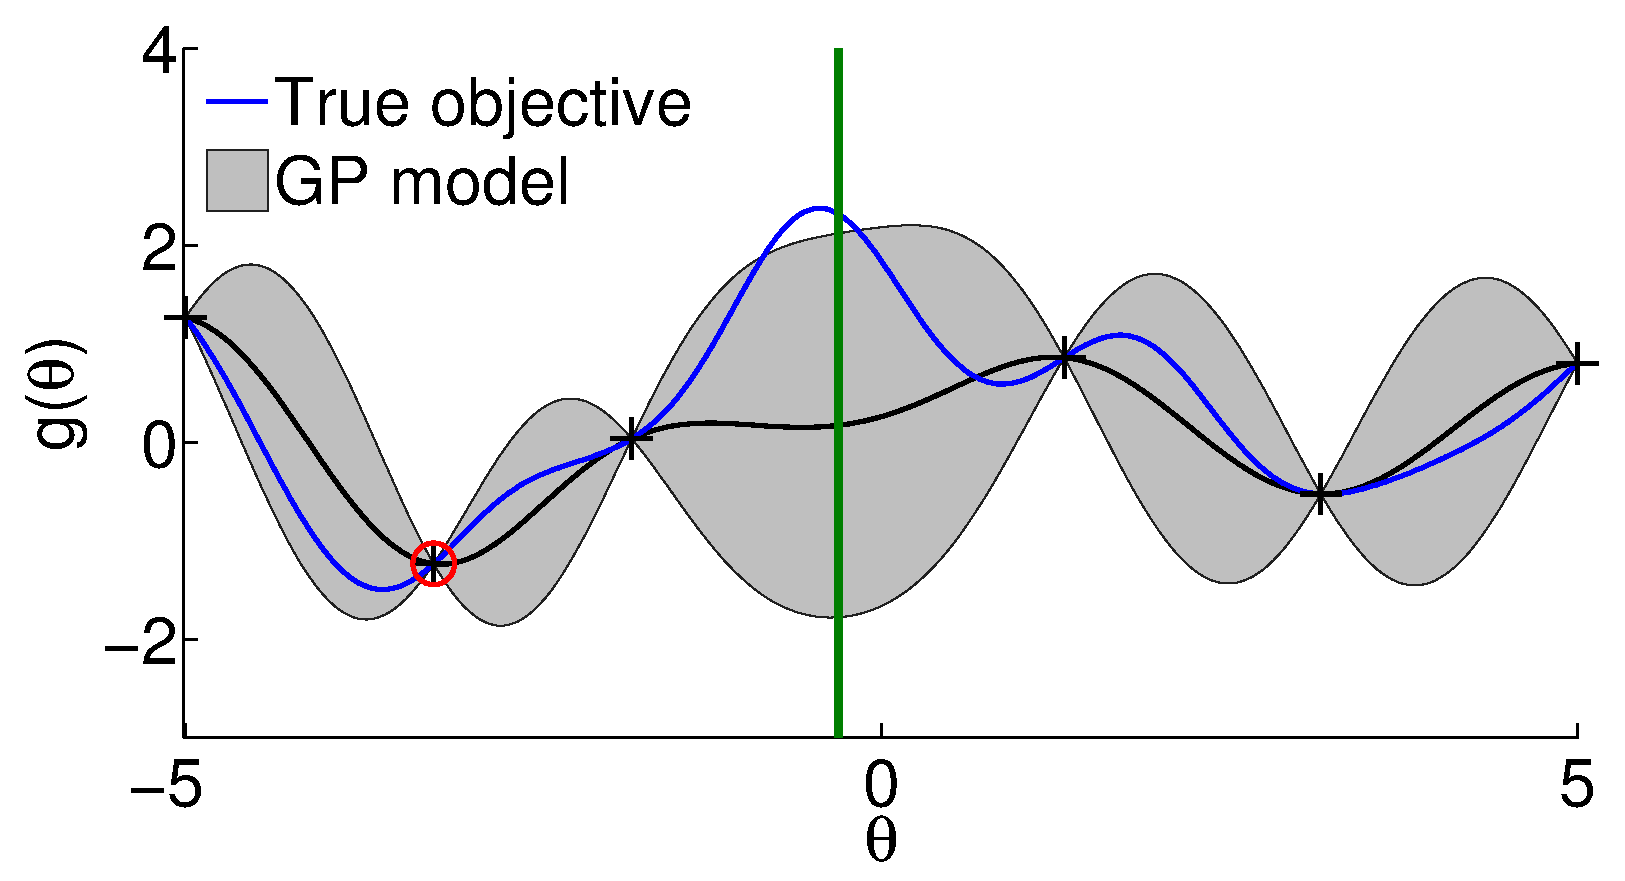
\includegraphics[height = 5cm]{./figures/bayesopt/BOb6}
\end{figure}
}
\onslide*<13>{
\begin{figure}
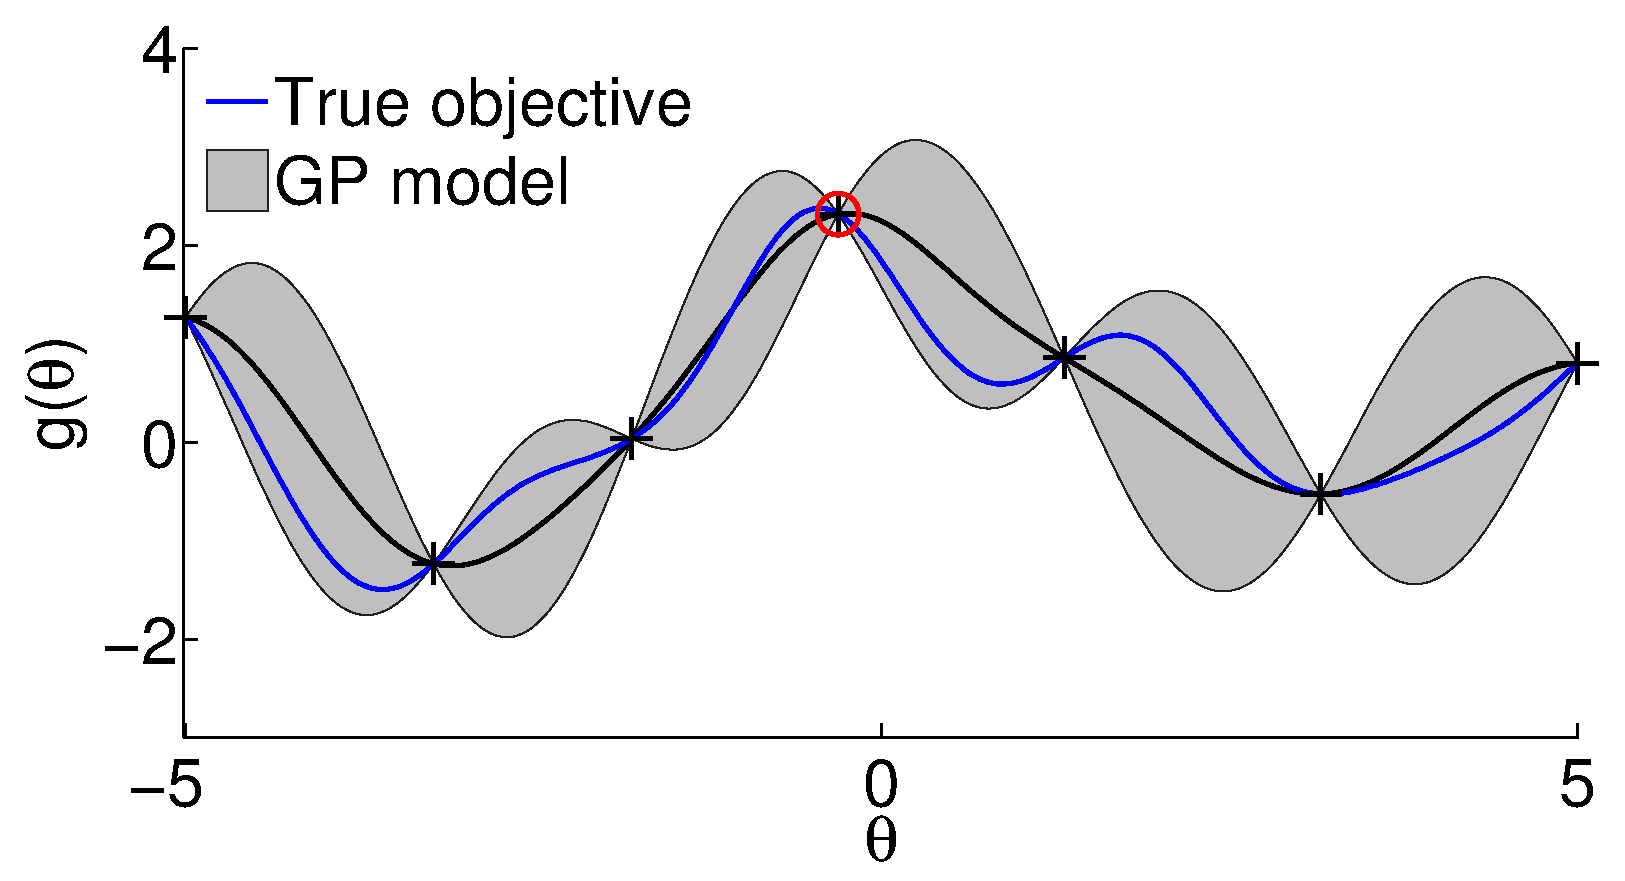
\includegraphics[height = 5cm]{./figures/bayesopt/BOa7}
\end{figure}
}
\onslide*<14>{
\begin{figure}
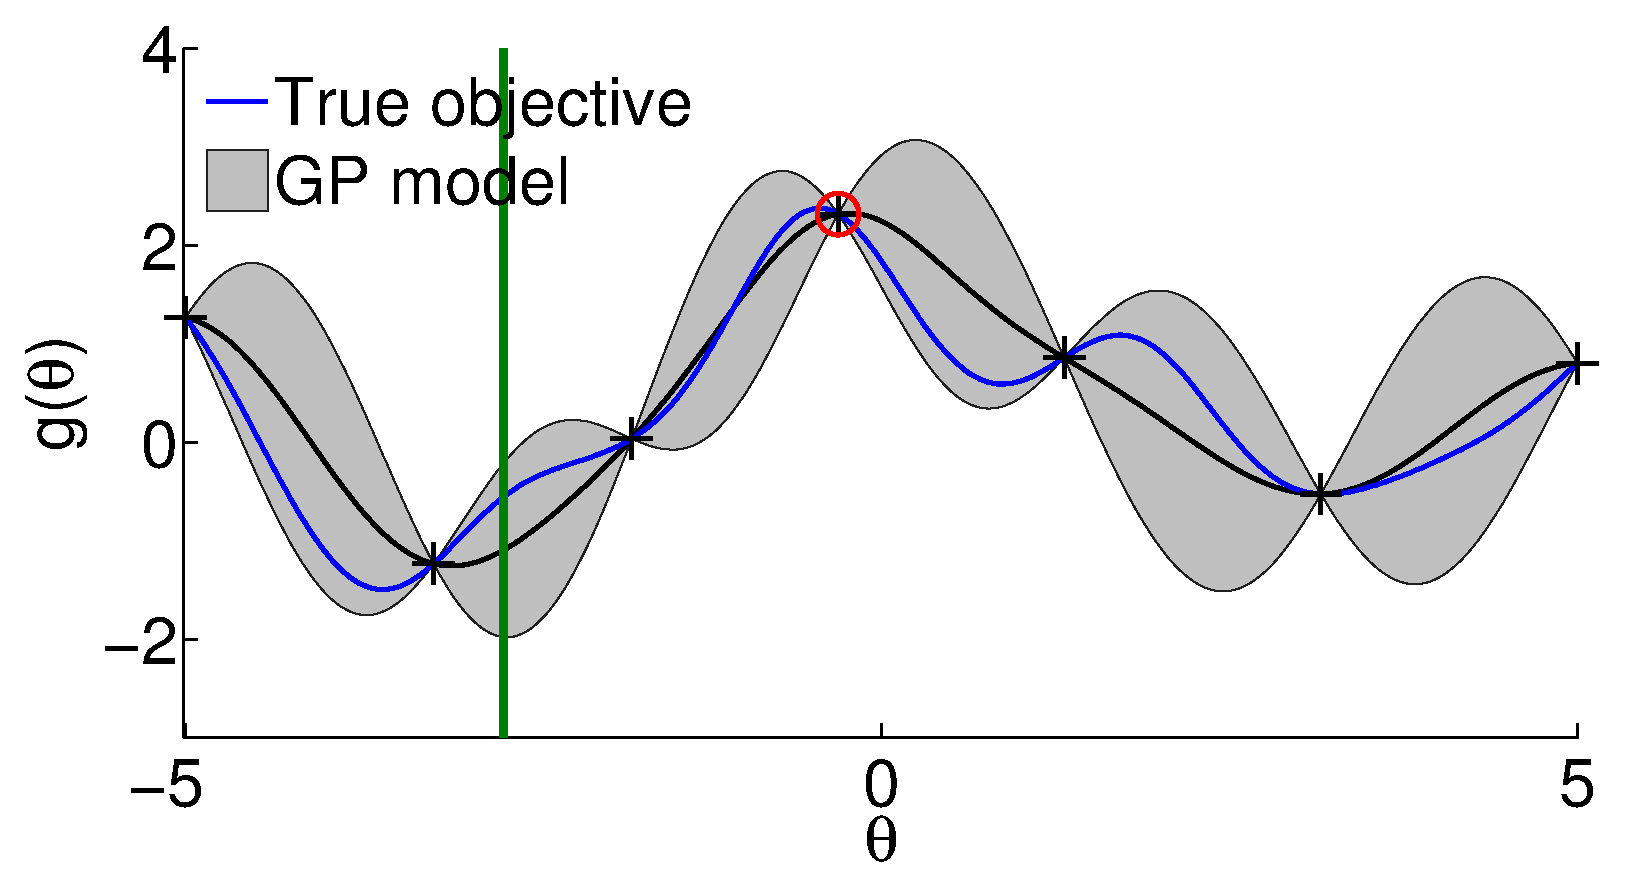
\includegraphics[height = 5cm]{./figures/bayesopt/BOb7}
\end{figure}
}
\onslide*<15>{
\begin{figure}
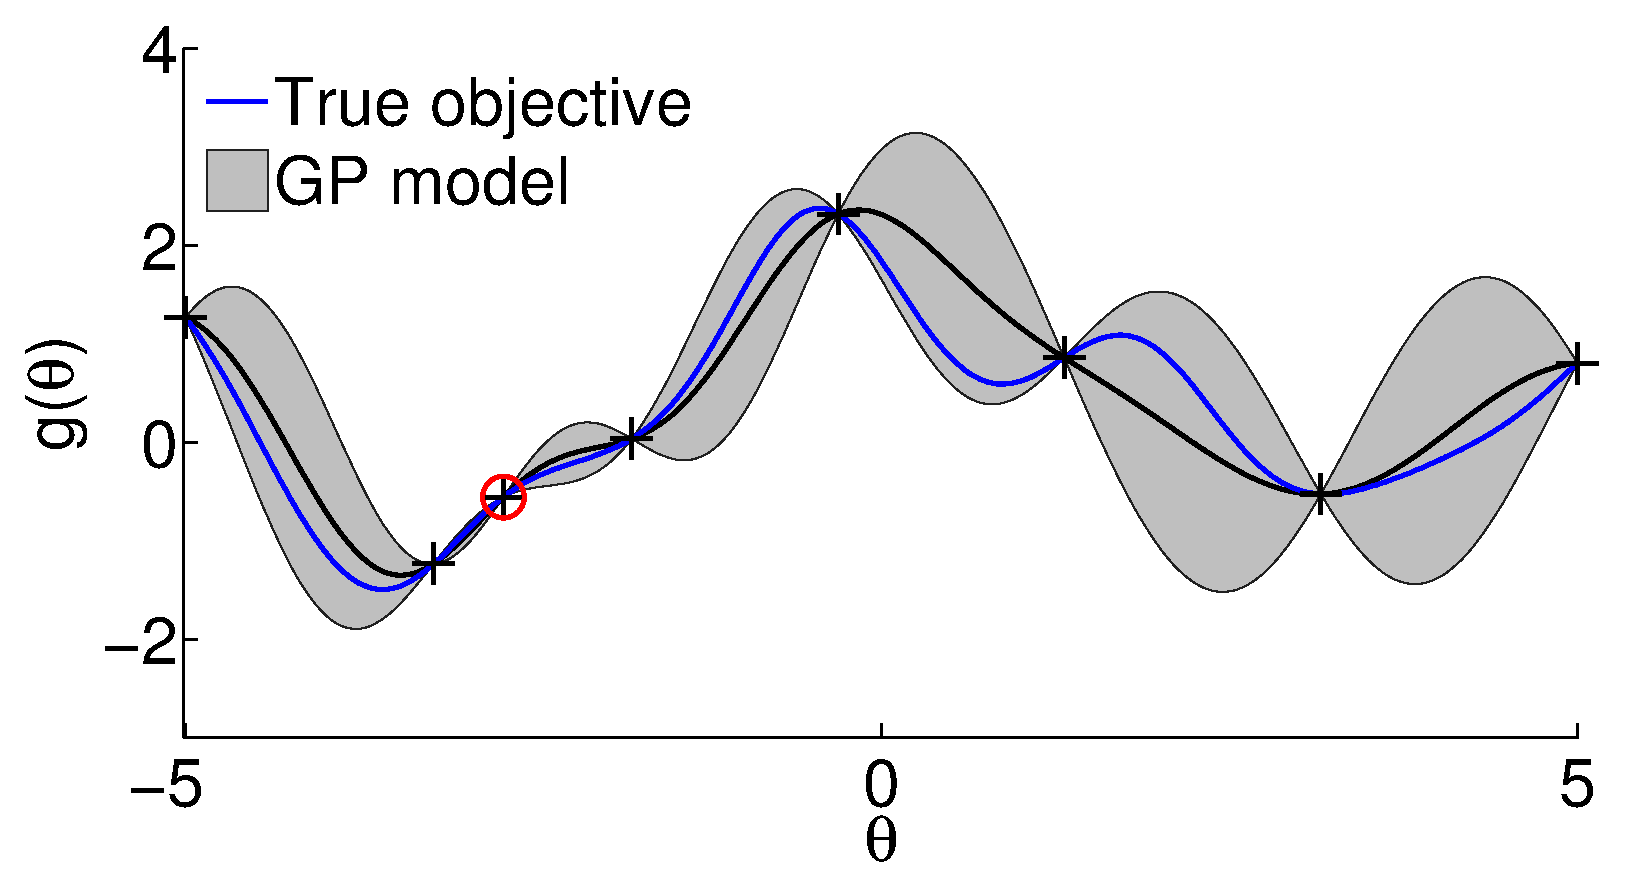
\includegraphics[height = 5cm]{./figures/bayesopt/BOa8}
\end{figure}
}
\onslide*<16>{
\begin{figure}
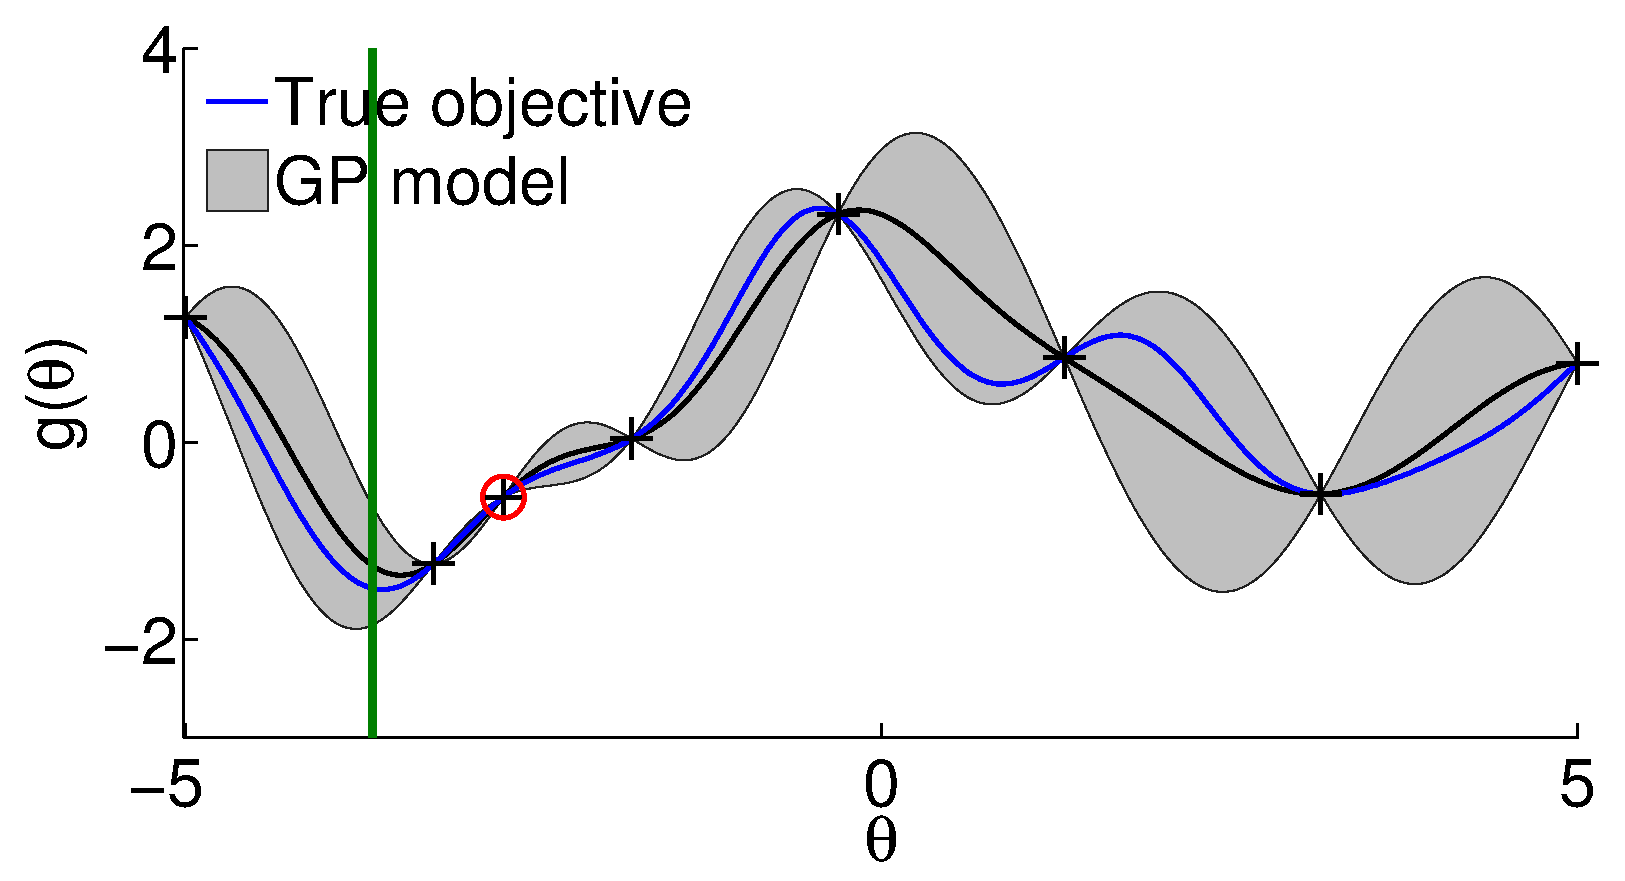
\includegraphics[height = 5cm]{./figures/bayesopt/BOb8}
\end{figure}
}
\onslide*<17>{
\begin{figure}
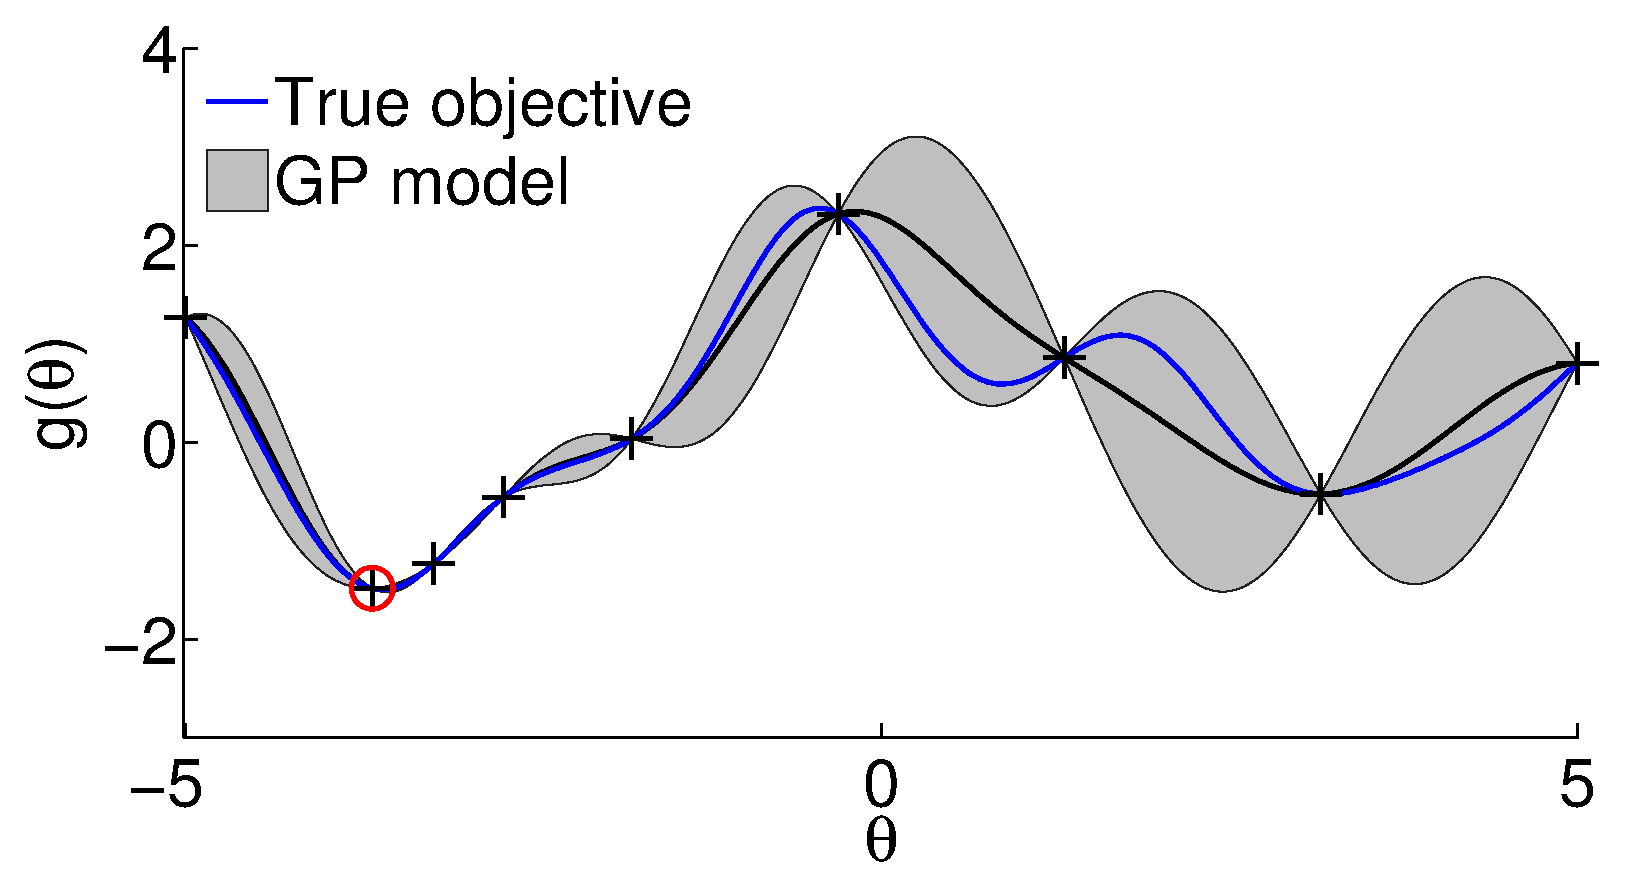
\includegraphics[height = 5cm]{./figures/bayesopt/BOa9}
\end{figure}
}
\onslide*<18>{
\begin{figure}
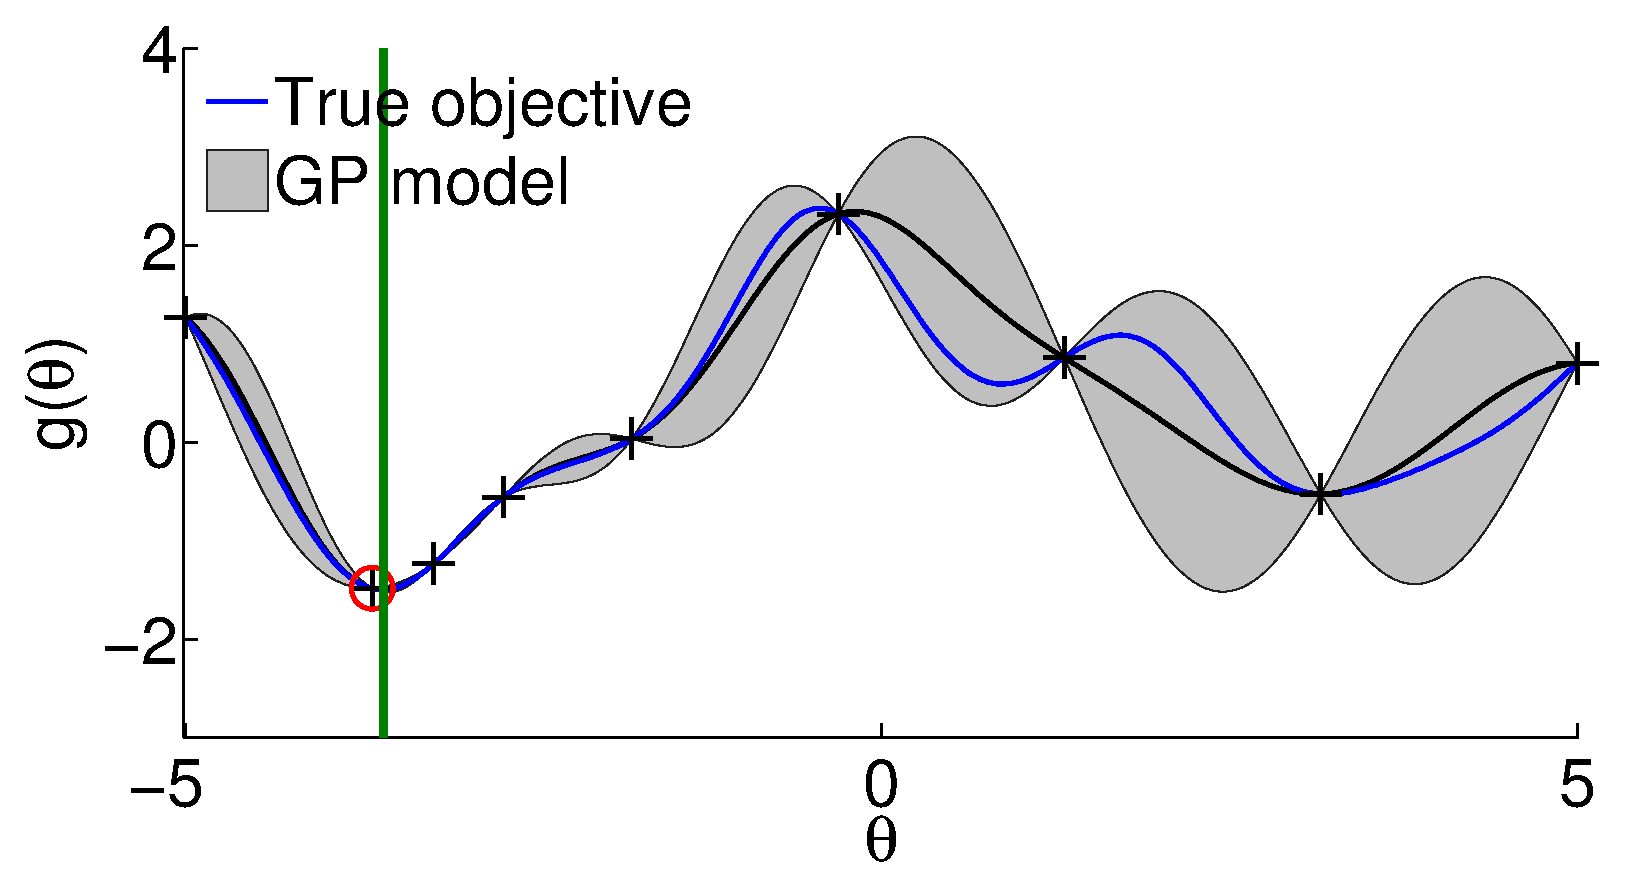
\includegraphics[height = 5cm]{./figures/bayesopt/BOb9}
\end{figure}
}
\onslide*<19>{
\begin{figure}
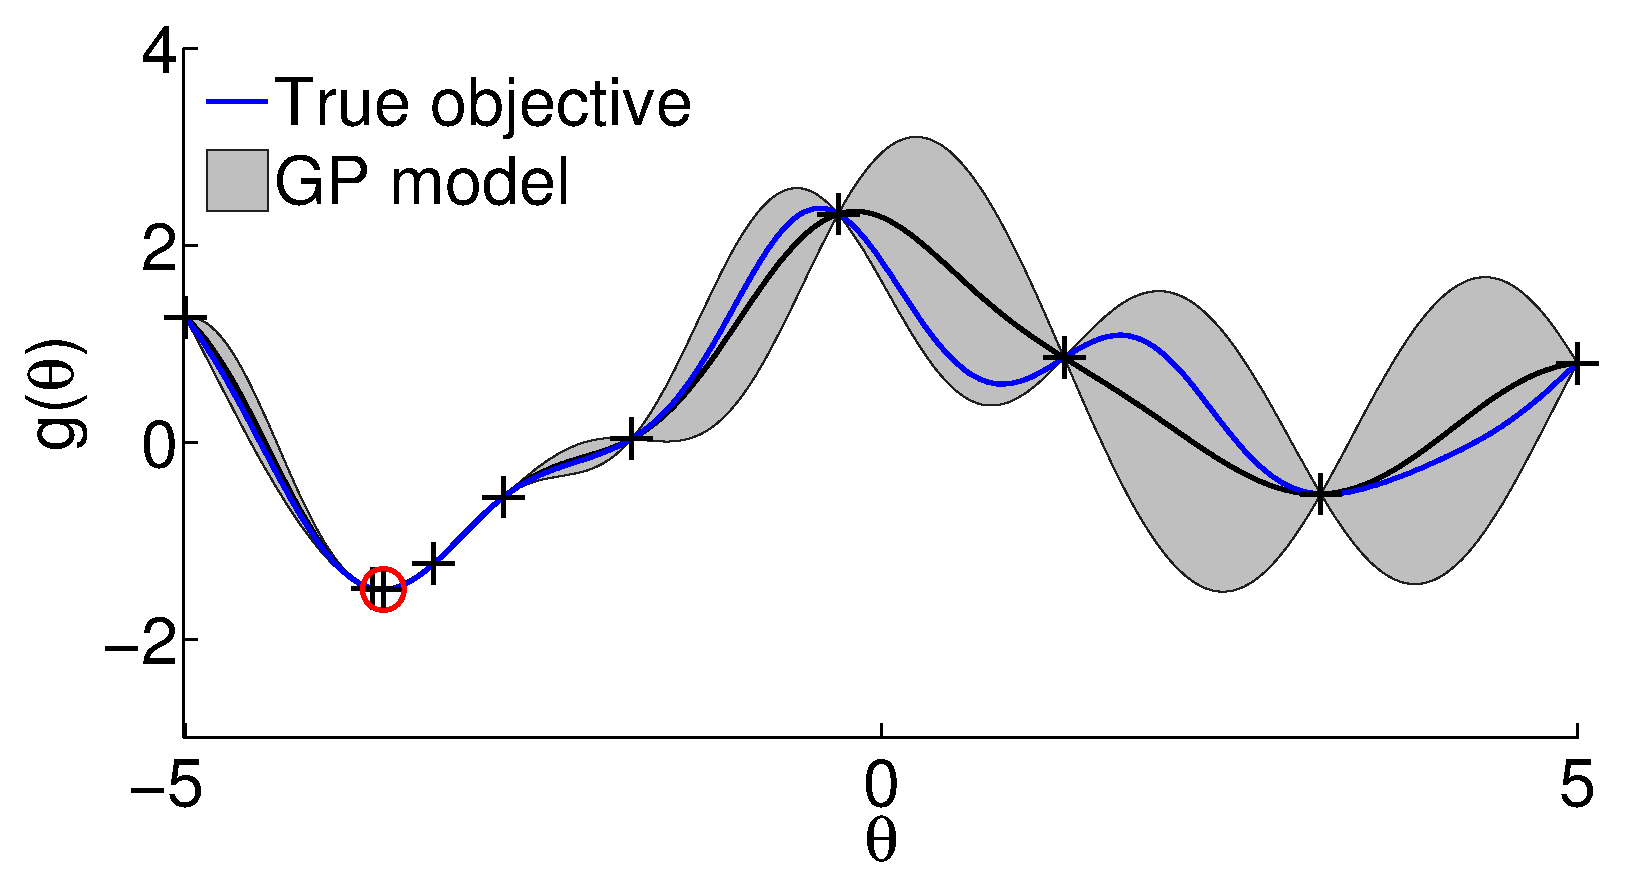
\includegraphics[height = 5cm]{./figures/bayesopt/BOa10}
\end{figure}
}
\onslide*<20>{
\begin{figure}
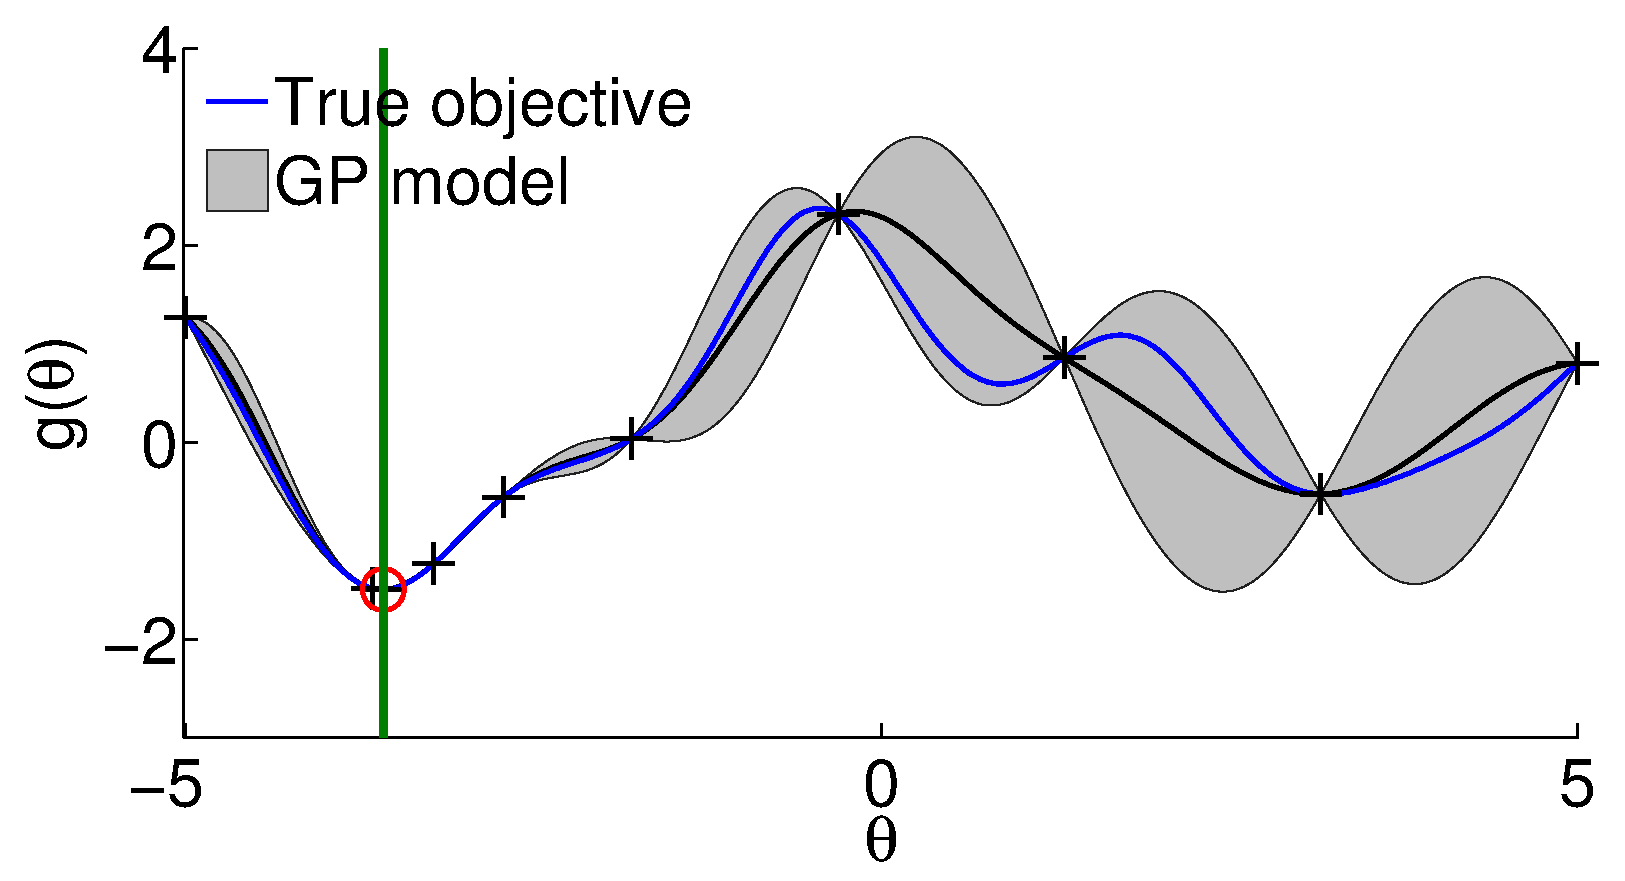
\includegraphics[height = 5cm]{./figures/bayesopt/BOb10}
\end{figure}
}
\onslide*<21>{
\begin{figure}
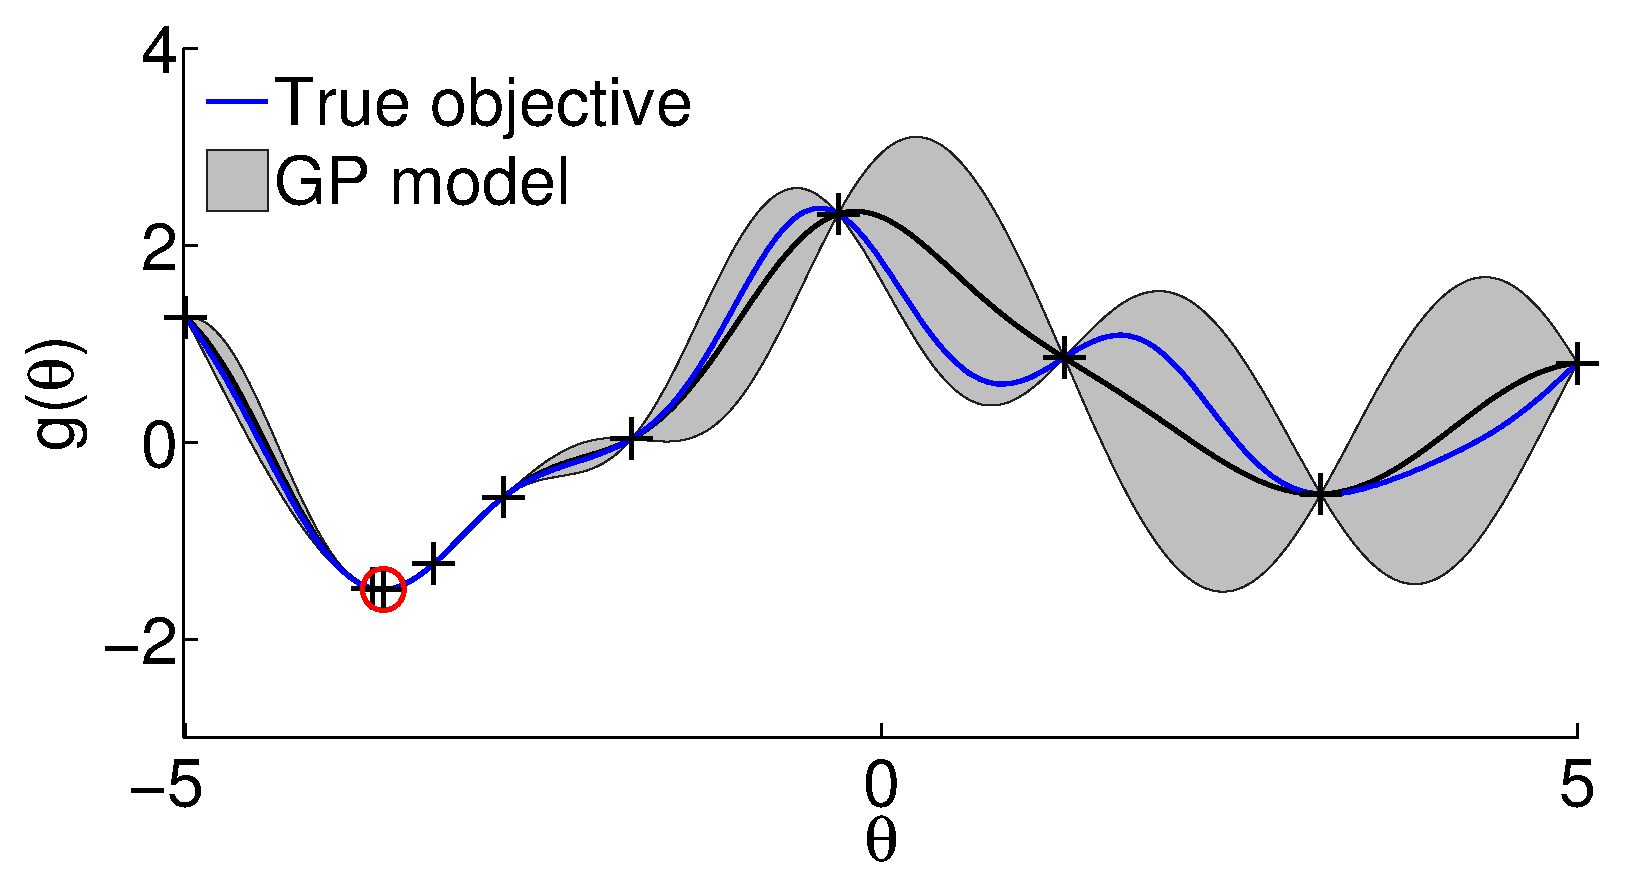
\includegraphics[height = 5cm]{./figures/bayesopt/BOa11}
\end{figure}
}
\onslide*<22>{
\begin{figure}
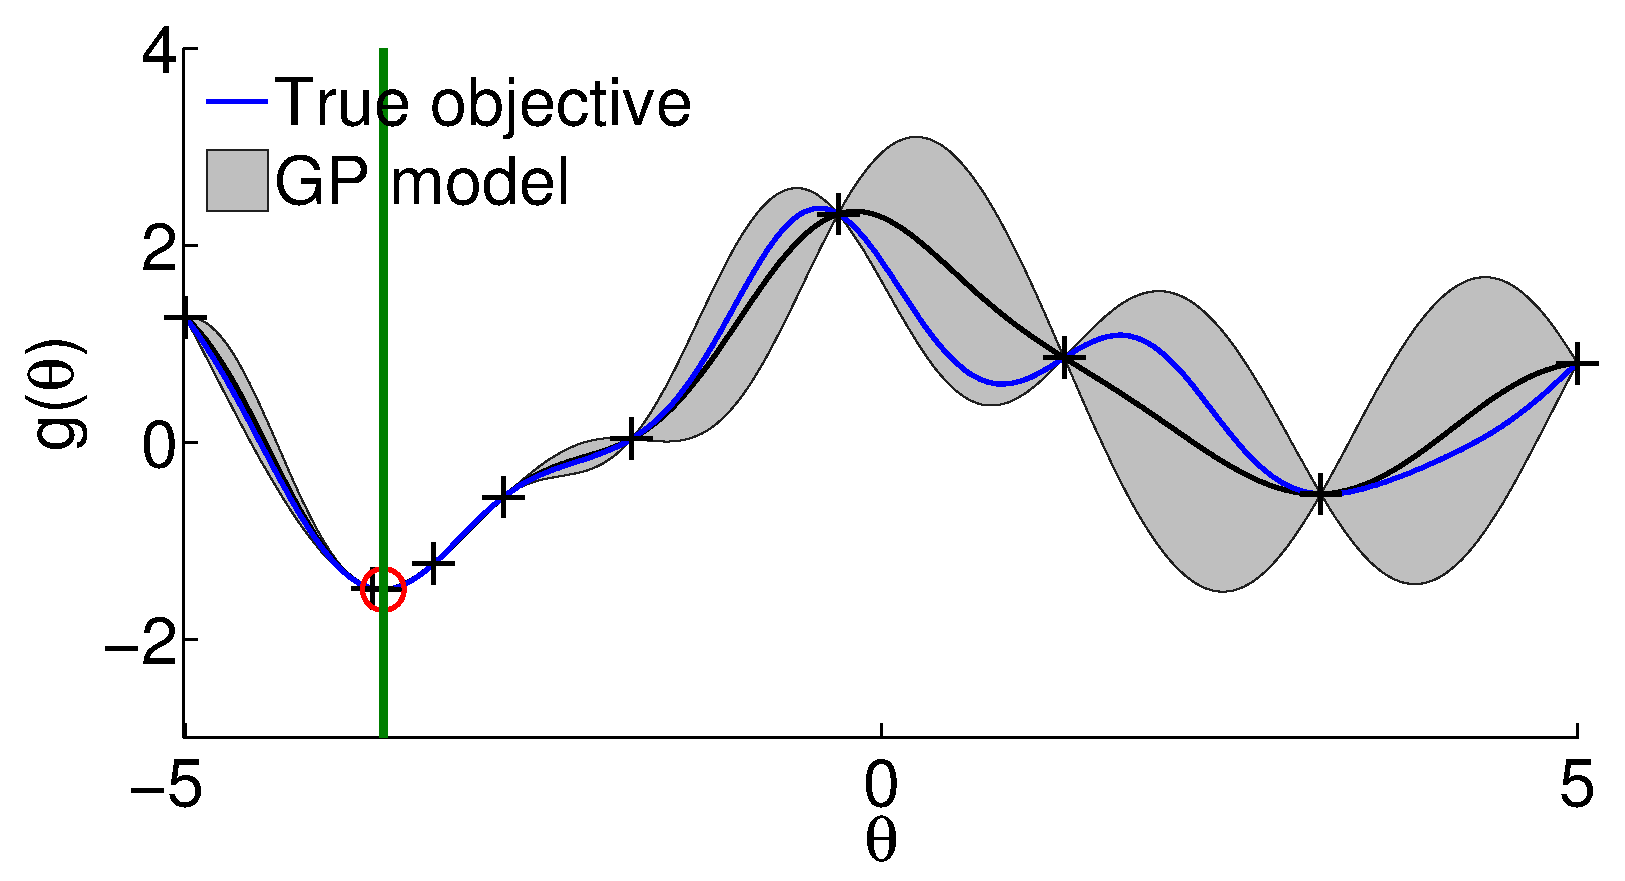
\includegraphics[height = 5cm]{./figures/bayesopt/BOb11}
\end{figure}
}
%
%
% \begin{itemize}
% \item \cemph{Lower-Confidence-Bound} (LCB) criterion to select next point
% $$
% \theta^* \in \arg\min_{\theta} \quad\E[\tilde g(\theta)] -
% 2\sqrt{\var[\tilde g(\theta)]}
% $$
% %\onslide+<22->{
% \only<22>{\item Global minimum found after 10 function evaluations}
% %}
% \phantom{1}
% \end{itemize}


\end{frame}









%%%%%%%%%%%%%%%%%%%%%%%%%%%%%%%%%%%%%%%%%%%%%%%%%%%%%

\begin{frame}
\frametitle{Optimising the Acquisition Function}
Notice: Acquisition function is multi-modal \pause
\begin{itemize}
\item Optimizing the acquisition function \calert{requires us to run a global
  optimizer inside Bayesian optimization}
\item What have we gained?
\pause
\item Evaluating the acquisition function is cheap compared to
  evaluating the true objective\\
\arrow We can afford evaluating it many times \\
\arrow Apply the usual tricks of many random restarts
\end{itemize}

% \begin{figure}
%   \centering
% 
\includegraphics[height = 2.1cm]{./figures/bayesopt/netflix}
% \hspace{5mm}
% 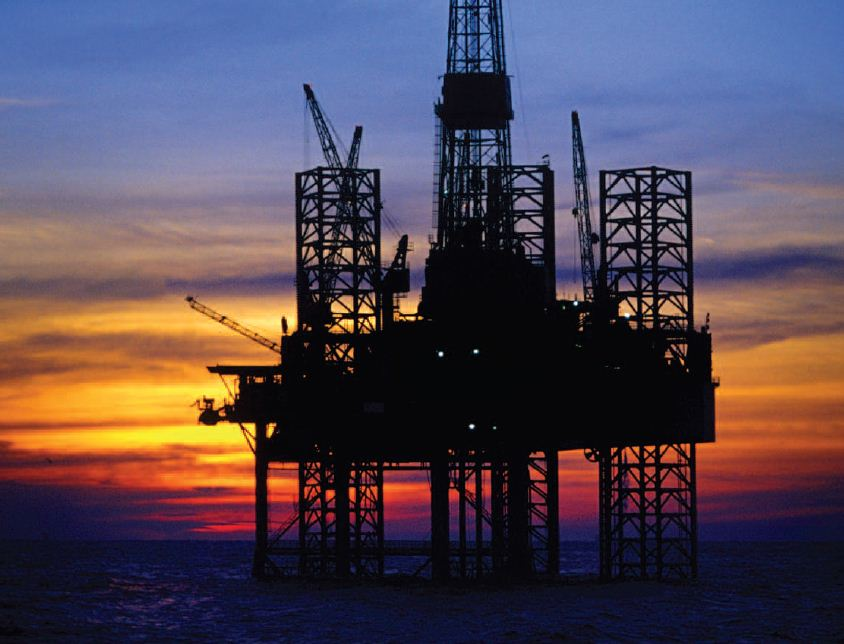
\includegraphics[height = 2.1cm]{./figures/bayesopt/oil}
% \hspace{5mm}
% 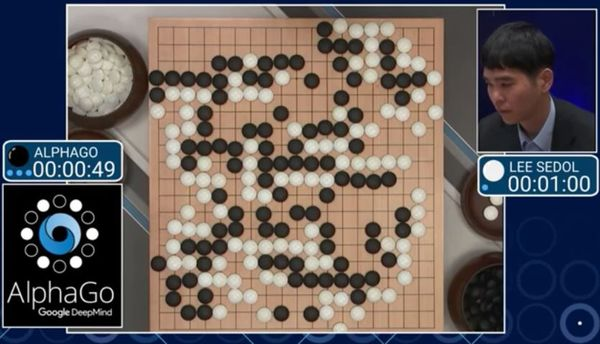
\includegraphics[height = 2.1cm]{./figures/bayesopt/alphago}\nocite{Chen2018}
% \end{figure}

\end{frame}



\begin{frame}
\frametitle{Key Steps (Pseudo-Code)}
\begin{algorithmic}[1]
\State \textbf{Init:} Data set $\mathcal D_0 = \{\mat X_0, \vec y_0\}$ (can be empty)
\For {iterations $t=1, 2, ...$}
\State \cemph{Update GP} using data $\mathcal D_{t-1}$
\State Select $\vec x_{t} = \arg\max_{\vec x} \alpha(\vec x)$ by
\cemph{optimising acquisition function}
\State Query true objective $g$ at $\vec x_{t}$
\State Augment data set $\mathcal D_{t} = \mathcal D_{t-1} \cup \{(\vec
x_{t}, y_{t})\}$
\EndFor
\State \textbf{Return} best input in data set: $\vec x^* = \arg\min_{\vec x} y(\vec x)$
\end{algorithmic}

Optimising acquisition function is itself an iterative process, done with a numerical gradient-based optimiser (e.g.~BFGS).
\end{frame}



\begin{frame}
\frametitle{Limitations}
\begin{itemize}
\item Getting the function model (e.g., covariance function) wrong can
  be catastrophic \pause
\begin{itemize}
\item Model will not correctly predict where function is high
\item Over/under estimation of uncertainty will lead to over/under exploration
\end{itemize}
\pause
\item Limited scalability in the number of dimensions and/or
  evaluations of the true
  objective function\\ \pause
\begin{itemize}
\item Local kernels too uncertain in high dimensions
\item Gaussian processes expensive for large datasets \pause (although BayesOpt generally doesn't have the problem of large datasets...)
\end{itemize}
\end{itemize}
\end{frame}

%%%%%%%%%%%%%%%%%%%%%%%%%%%%%%%%%%%%%%%%%%%%%%%%%%%%%
\begin{frame}
\frametitle{Poor Model Choice}
\begin{figure}
\centering
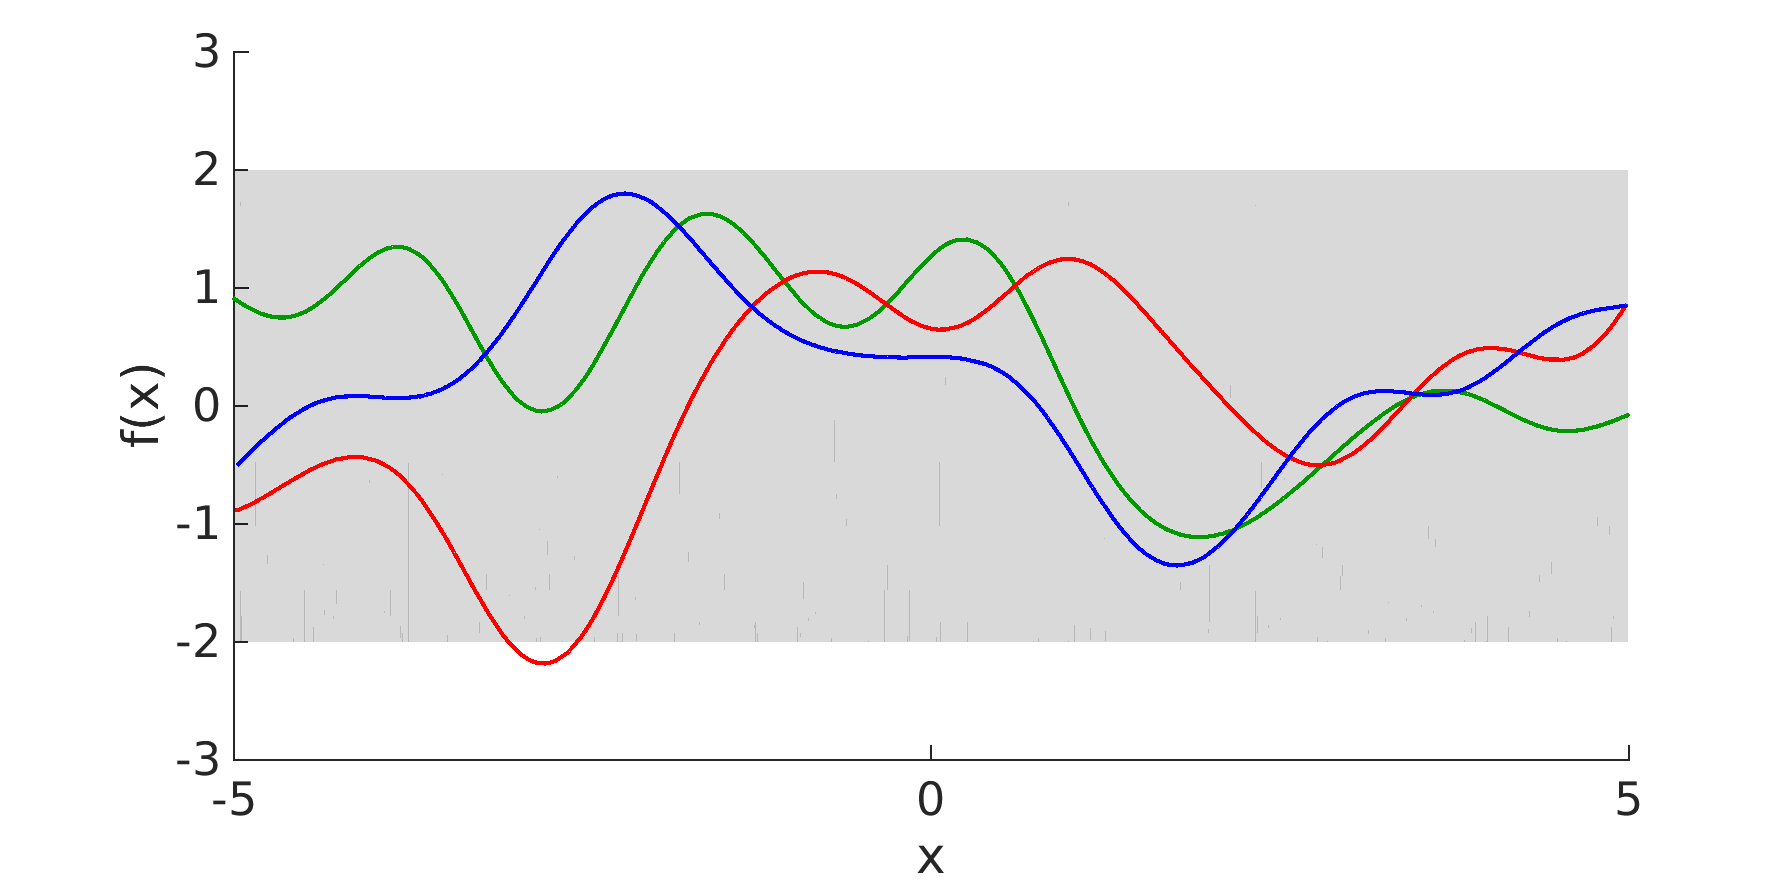
\includegraphics[width = 0.48\hsize]{./figures/bayesopt/samplesGauss}
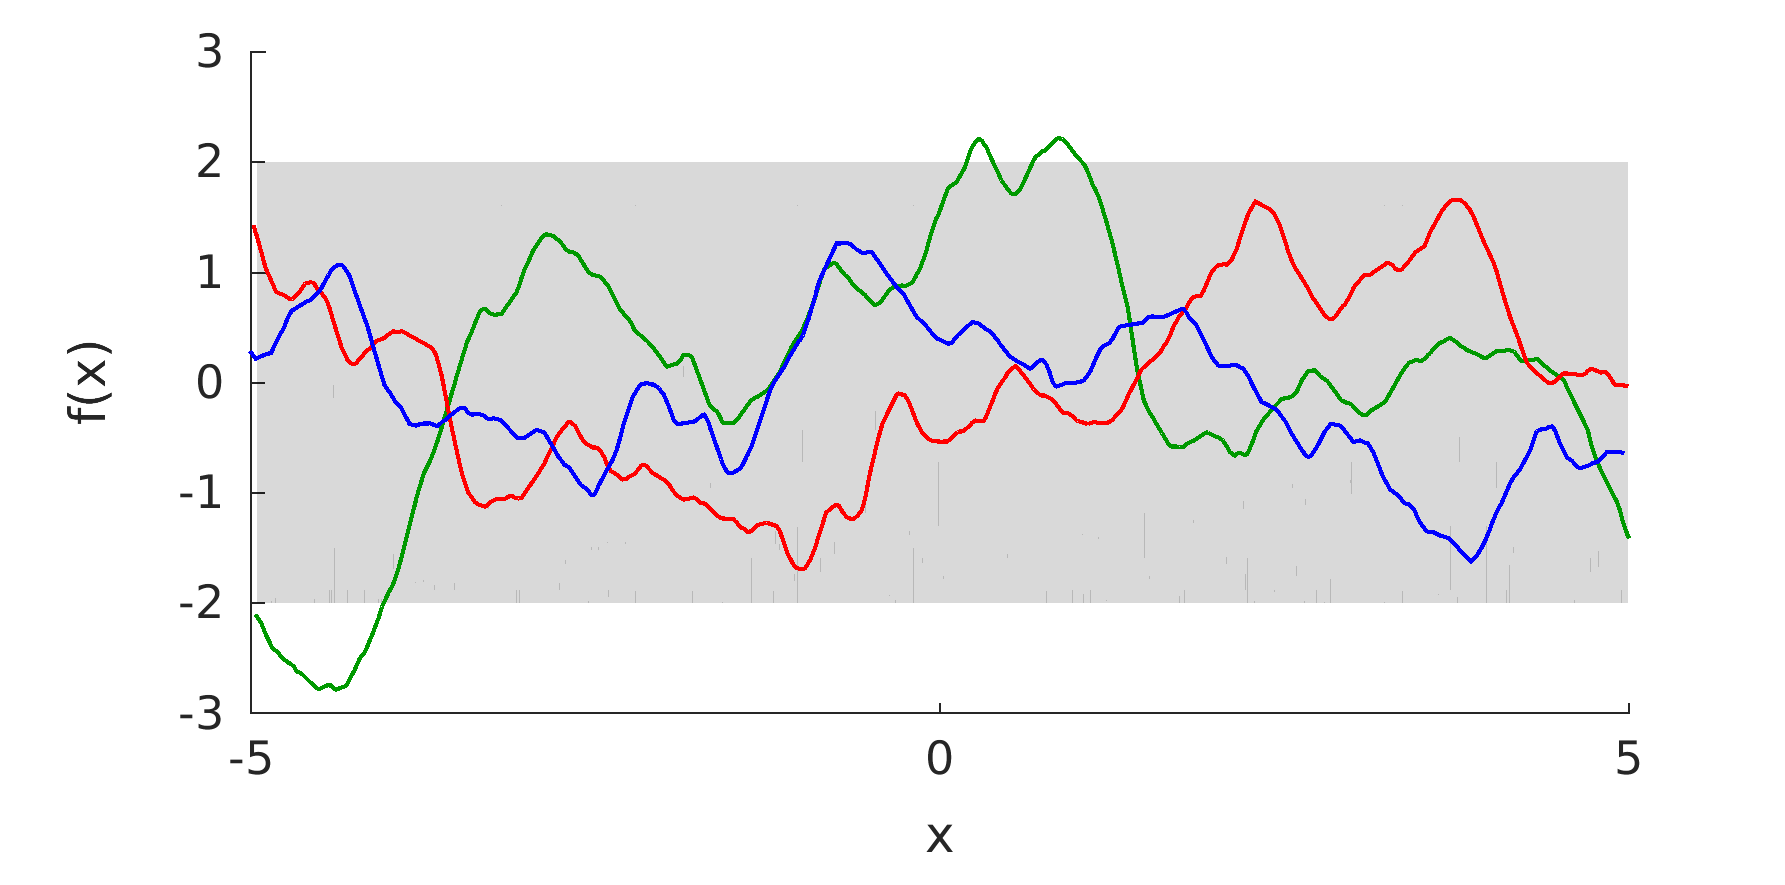
\includegraphics[width = 0.48\hsize]{./figures/bayesopt/samplesMatern3}
\end{figure}

\begin{itemize}
\item Covariance function selection is crucial for good performance\\
\arrow Choose a sufficiently flexible and adaptive kernel, e.g.,
Mat\'ern (but not the squared exponential (Gaussian))
\pause
\item Nice side-effect of Mat\'ern: Exploration is more encouraged than with
  the Gaussian kernel
\end{itemize}

\end{frame}
%%%%%%%%%%%%%%%%%%%%%%%%%%%%%%%%%%%%%%%%%%%%%%%%%%%%%
\begin{frame}
\frametitle{Choosing Covariance Functions}
Application:
\begin{itemize}
\item Structured SVM for Protein Motif Finding (Miller et al.,
2012)\nocite{Miller2012}
\item  Optimize hyper-parameters of SSVM using
BO (Snoek et al., 2012)\nocite{Snoek2012}
\end{itemize}
\begin{figure}
\centering
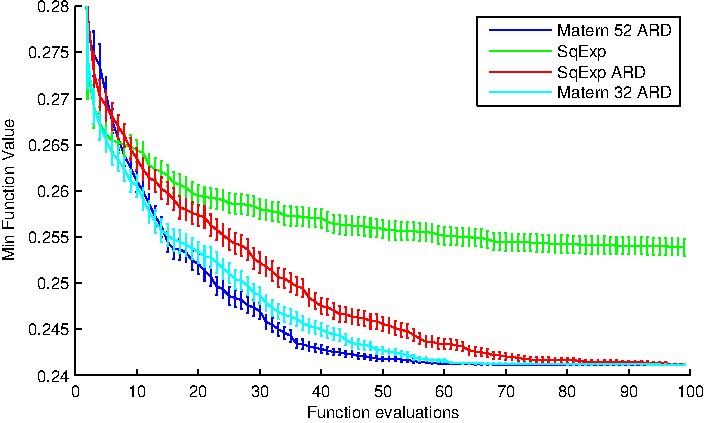
\includegraphics[width = 0.68\hsize]{./figures/bayesopt/ssvmmotif_comparison_kernel}
\caption{Figure from Snoek et al. (2012)~\nocite{Snoek2012}}
\end{figure}



\end{frame}



%%%%%%%%%%%%%%%%%%%%%%%%%%%%%%%%%%%%%%%%%%%%%%%%%%%%%

\begin{frame}
\frametitle{Gaussian Process Hyper-Parameters}
\begin{itemize}[<+->]
\item \calert{Empirical Bayes (maximize the marginal likelihood) can fail
  horribly,} especially in the early stages of Bayesian optimization
  when we have only a few data points
\item Solution: Integrate out the GP hyper-parameters $\vec\theta$ by \cemph{Markov Chain
  Monte Carlo (MCMC)} sampling (e.g., slice sampling)
\item Look at \cemph{integrated acquisition function}
\begin{align*}
\alpha(\vec x) &= \E_{\vec \theta}[\alpha(\vec x, \vec\theta)] = \int \alpha(\vec x,\vec\theta)p(\vec\theta)
  d\vec\theta\\
&\approx \frac{1}{K}\sum_{k=1}^K \alpha(\vec
  x,\vec\theta^{(k)})\,,\quad \vec\theta^{(k)}\sim\hspace{-5mm}
  \underbrace{p(\vec\theta|\mat X_n, \vec y_n)}_{\text{hyper-parameter
  posterior}}
\end{align*}
\end{itemize}
\end{frame}
%%%%%%%%%%%%%%%%%%%%%%%%%%%%%%%%%%%%%%%%%%%%%%%%%%%%%
\begin{frame}
\frametitle{Integrating out GP Hyper-parameters}
\begin{itemize}
\item Online LDA (Hoffman et al., 2010)~\nocite{Hoffman2010} for topic
  modeling
\item Two critical hyper-parameters that control the learning rate
  learned by BO (Snoek et al., 2012) \nocite{Snoek2012}
\end{itemize}
\begin{figure}
\centering
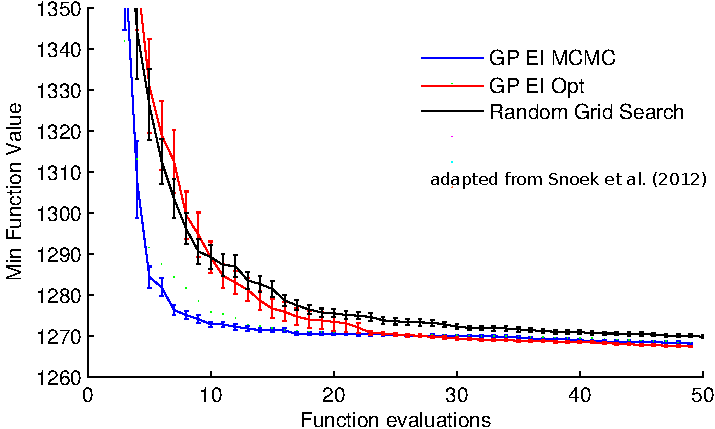
\includegraphics[width = 0.68\hsize]{./figures/bayesopt/onlinelda_comparison}
\caption{Figure from Snoek et al. (2012)~\nocite{Snoek2012}}
\end{figure}

\end{frame}


%%%%%%%%%%%%%%%%%%%%%%%%%%%%%%%%%%%%%%%%%%%%%%%%%%%%%
\begin{frame}
\frametitle{Robots That Learn to Recover from Damage}
\begin{figure}
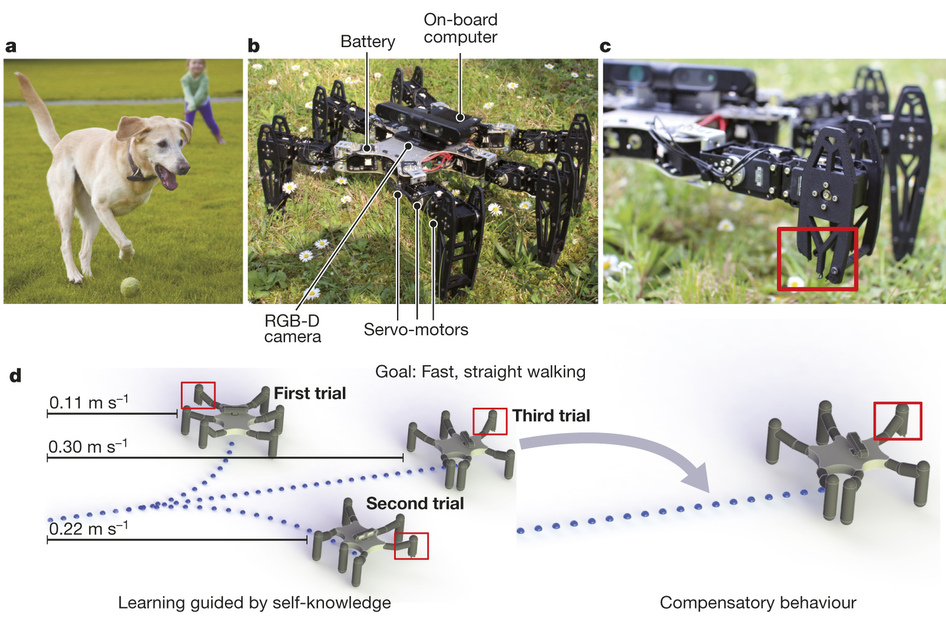
\includegraphics[width = 0.9\hsize]{./figures/bayesopt/robot_fix_learn}
\\
Cully et al. (2015)\nocite{Cully2015}
\end{figure}
\end{frame}


%%%%%%%%%%%%%%%%%%%%%%%%%%%%%%%%%%%%%%%%%%%%%%%%%%%%%

\begin{frame}
\frametitle{Application Example: Controller Learning in Robotics
  {\small (Calandra et al., 2015)}}
\begin{minipage}[t]{0.65\hsize}
\begin{itemize}
\item Fragile bipedal robot \\
\arrow Only few experiments feasible
\item Maximize robustness and walking speed
\item 4 motors: \\
2 actuated hips + 2 actuated knees
\item Controller implemented as a finite-state-machine (8 parameters)
\onslide+<2->{
\item Good parameters found after 80--100 experiments
\item \cemph{Substantial speed-up} compared to manual parameter search
}
\end{itemize}
\end{minipage}
\begin{minipage}[t]{0.3\hsize}
\begin{figure}
\centering
 \movie[externalviewer, poster]{\includegraphics[height =
  4.5cm]{./figures/bayesopt/fox}}{/home/marc/research/svn/marc/videos/fox_gait_optimization_summary_short.mpeg}
\\
{\small Calandra et al. (2015)\nocite{Calandra2015a}}
\end{figure}
\end{minipage}
%

\end{frame}
%%%%%%%%%%%%%%%%%%%%%%%%%%%%%%%%%%%%%%%%%%%%%%%%%%%%%
\begin{frame}
\frametitle{Comparison}
\begin{figure}
\centering
\includegraphics[height = 4cm]{./figures/bayesopt/fox_opt_curves}
\end{figure}


\begin{itemize}
\item Squared exponential covariance function
\item Learned GP hyper-parameters (no MCMC for integrating them out)
\end{itemize}

\end{frame}



% %%%%%%%%%%%%%%%%%%%%%%%%%%%%%%%%%%%%%%%%%%%%%%%%%%%%%
%
% \begin{frame}
% \frametitle{Applications}
% \nocite{Calandra2015a, Lizotte2008, Martinez-Cantin2007}
% \begin{itemize}
% \item Robotics
% \item Cheetah robot
% \item Training neural networks
% \item Optimizing simulators
% \item Wetlab and Twitter
% \end{itemize}
%
% \end{frame}
%%%%%%%%%%%%%%%%%%%%%%%%%%%%%%%%%%%%%%%%%%%%%%%%%%%%%
\begin{frame}
\frametitle{Further Topics in BO}

\begin{itemize}
\item \cemph{Entropy-based acquisition functions:} Directly describe the distribution over the best input location (Hennig \& Schuler, 2012; Hern\'andez-Lobato et al., 2014)
\item \cemph{Non-myopic} Bayesian optimization (e.g., Osborne et al., 2009)\nocite{Osborne2009}
\item \cemph{High-dimensional} optimization (e.g., Wang et al., 2016)\nocite{Wang2016}
\item \cemph{Large-scale} Bayesian optimization (Hutter et al., 2014)\nocite{Hutter2014}
\item \cemph{Efficient optimization of acquisition functions} (Wilson et al., 2018)\nocite{Wilson2018}
\item \cemph{Non-GP} Bayesian optimization (Hutter et al., 2014; Snoek et al.,
  2015)\nocite{Jones1998, Hutter2014,Snoek2015, Springenberg2016}
\item \cemph{Constraints} (e.g., Gelbart et al., 2014)\nocite{Gelbart2014}
\item \cemph{Automated machine learning} (e.g., Feurer et al.,
  2015)\nocite{Feurer2015}
\item \cemph{Multi-tasking, parallelizing, resource allocation}, ... (e.g.,
  Swersky et al., 2014; Snoek et al., 2012; Wilson et al., 2018)\nocite{Swersky2014, Snoek2012}

\end{itemize}



\end{frame}

%%%%%%%%%%%%%%%%%%%%%%%%%%%%%%%%%%%%%%%%%%%%%%%%%%%%%
\begin{frame}
\frametitle{Software}
\begin{itemize}
\item \cemph{BayesOpt} \url{https://bitbucket.org/rmcantin/bayesopt/}
  (Martinez-Cantin, 2014)\nocite{Martinez-Cantin2014}
\item \cemph{Spearmint} \url{https://github.com/HIPS/Spearmint}
\item \cemph{Pybo} \url{https://github.com/mwhoffman/pybo} (Hoffman \& Shariari)
\item \cemph{GPyOpt} \url{https://github.com/SheffieldML/GPyOpt}
  (Gonzalez et al.)
\item Matlab toolbox (bayesopt)
\end{itemize}
\end{frame}


%%%%%%%%%%%%%%%%%%%%%%%%%%%%%%%%%%%%%%%%%%%%%%%%%%%%%
\begin{frame}{Summary}

  \begin{figure}
    \centering
      \includegraphics[height=2.5cm]{./figures/bayesopt/protein}
  \hspace{5mm}
    \includegraphics[height = 2.5cm]{./figures/bayesopt/alphago}
    \hspace{5mm}
    \movie[externalviewer, poster]{\includegraphics[height =
  2.5cm]{./figures/bayesopt/fox}}{/home/marc/research/svn/marc/videos/fox_gait_optimization_summary_short.mpeg}
  \end{figure}
  
  
  \begin{itemize}
    \item Global optimization of black-box functions, which are
      expensive to evaluate
    %
      \arrow Meta-challenges in machine learning, Auto-ML
    \item Use a probabilistic proxy model that is cheap to evaluate
      and use this to suggest next experiments
    \item Acquisition function trades of exploration and exploitation
  \end{itemize}
  
\end{frame}









% \begin{frame}{Coursework}
% \begin{itemize}
% \item Part tutorial to guide you though a simple GP implementation
% \item Assessed part on Bayesian optimisation
% \item Submission through labts
% \item Will be released later today or tomorrow
% \item Full description on Piazza
% \end{itemize}
% \end{frame}


\begin{frame}{Further Reading}
  \begin{itemize}
  \item Brochu et al.: \textit{A Tutorial on Bayesian Optimization of
    Expensive Cost Functions, with Application to Active User Modeling
    and Hierarchical Reinforcement Learning}, arXiv:1012.2599, 2012
  \item Shahriari et al.: \textit{Taking the Human Out of the Loop: A Review
    of Bayesian Optimization}, Proceedings of the IEEE, 2016
  \end{itemize}
\end{frame}










%%%%%%%%%%%%%%%%%%%%%%%%%%%%%%%%%%%%%%%%%
% REFERENCES
%%%%%%%%%%%%%%%%%%%%%%%%%%%%%%%%%%%%%%%%%
\begin{frame}[t,allowframebreaks]
\frametitle{References}
\linespread{1.0}
\tiny
\bibliographystyle{abbrv}
\bibliography{../includes/pi-literature}
\end{frame}



\end{document}
%%% Local Variables: 
%%% mode: latex
%%% TeX-master: t
%%% End: 
